% -----------------------------------------------------------------
% -----------------------------------------------------------------
\subsection{Additional figures}\label{app:6:moreFigures}
% -----------------------------------------------------------------

We give here plots showing the mean regret $R_t$ as a function of time, and histograms of the distributions of the final regret $R_T$, for the different problems of our benchmark.

Figures~\ref{fig:6:meanRegretPb1} above and \ref{fig:6:histogramRegretPb1} below show that our two proposals are efficient against problem 1.
Then we show similar results for problem 2 in Figure~\ref{fig:6:meanRegretPb2}
and for problem 4 in Figure~\ref{fig:6:meanRegretPb4}.

% -----------------------------------------------------------------
\begin{figure}[h!]  % [htbp]
    \centering
    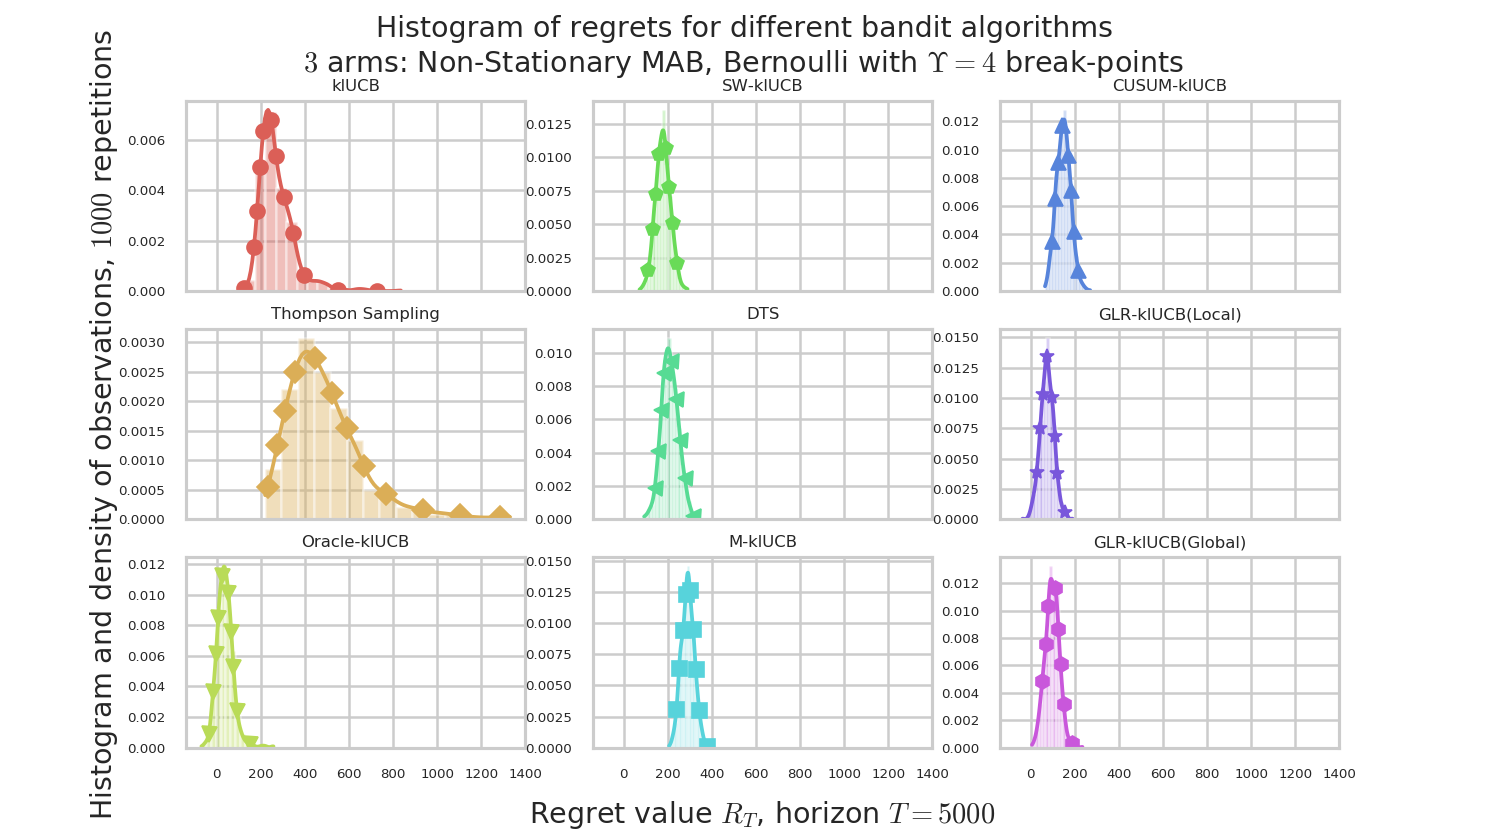
\includegraphics[width=1.09\linewidth]{2-Chapters/6-Chapter/nonstatbandits.git/figures/SP__K3_T5000_N1000__9_algos_pb1/main_HistogramsRegret_shareX____env1-1_1316297932259102962.pdf}
    \caption{Histograms of the distributions of regret $R_T$ ($T=5000$) for problem 1.}
    \label{fig:6:histogramRegretPb1}
\end{figure}

% -----------------------------------------------------------------
\begin{figure}[h!]  % [htbp]
    \centering
    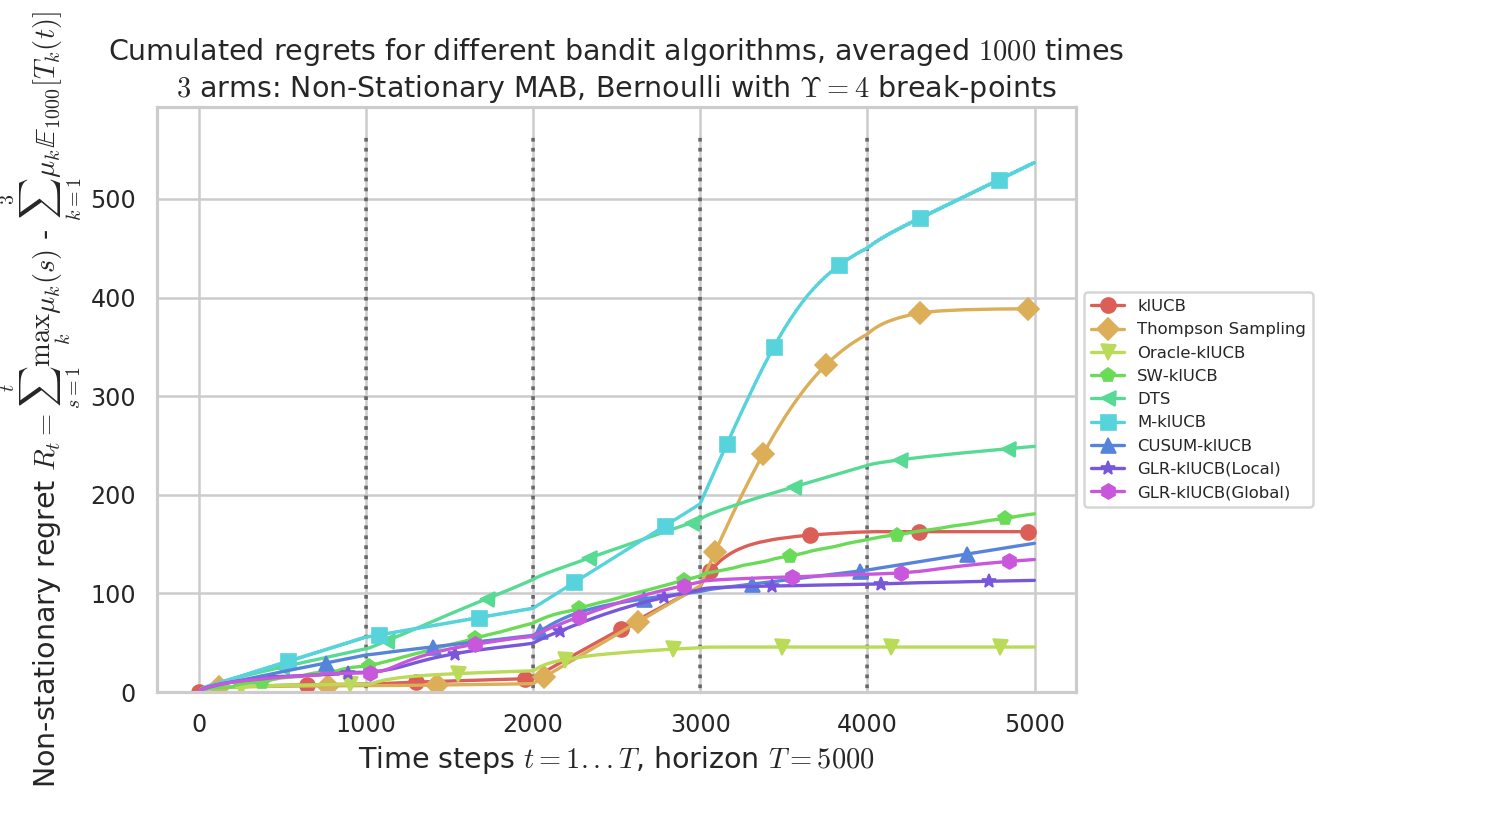
\includegraphics[width=1.09\linewidth]{2-Chapters/6-Chapter/nonstatbandits.git/figures/SP__K3_T5000_N1000__9_algos_pb2/main____env1-1_7882655236216606305.pdf}
    \caption{Mean regret as a function of time, $R_t$ ($1 \leq t \leq T = 5000$) for problem $2$.}
    \label{fig:6:meanRegretPb2}
\end{figure}

% -----------------------------------------------------------------
\begin{figure}[h!]  % [htbp]
    \centering
    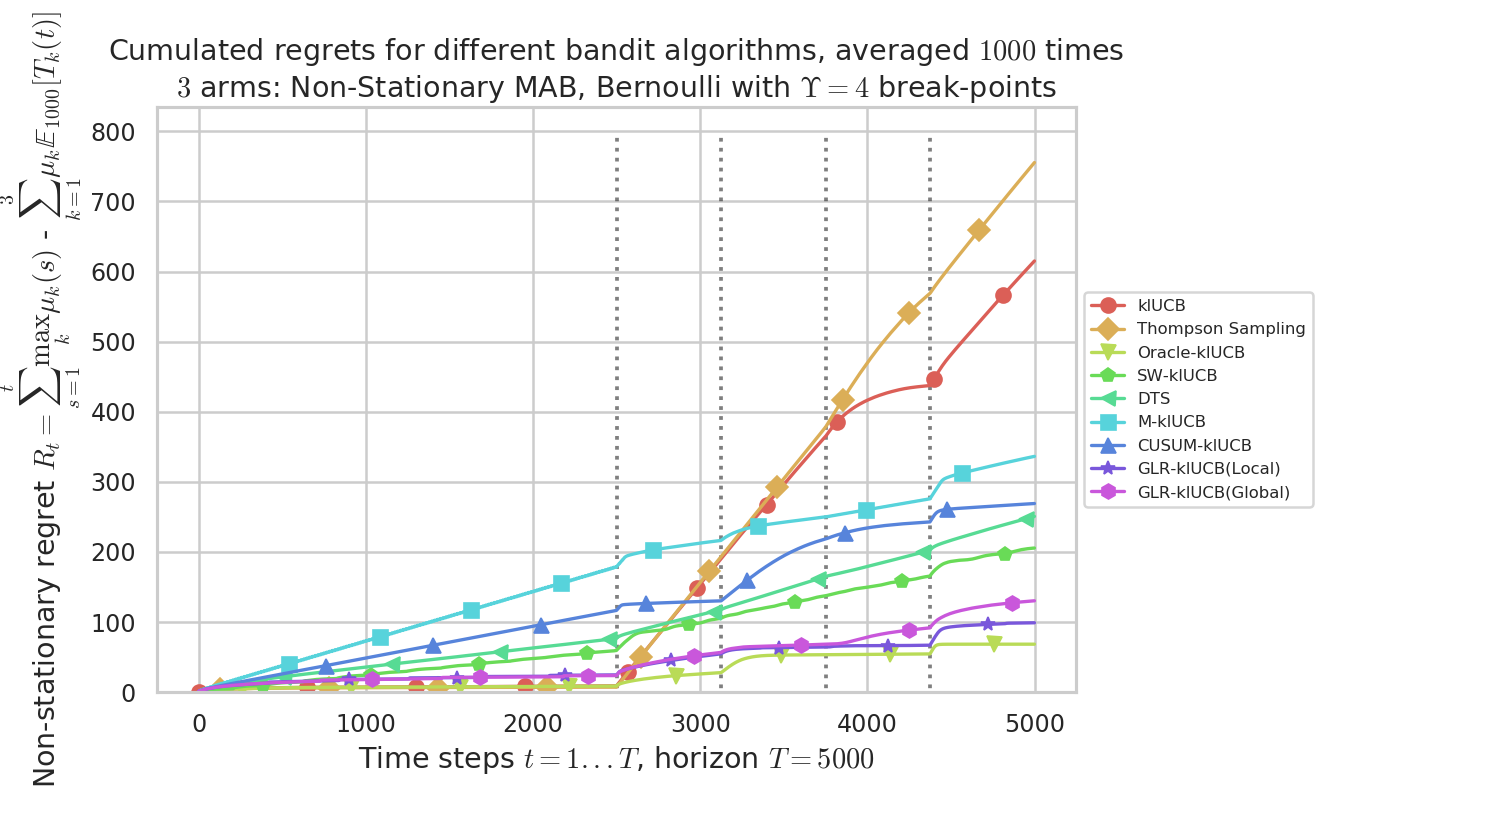
\includegraphics[width=1.09\linewidth]{2-Chapters/6-Chapter/nonstatbandits.git/figures/SP__K3_T5000_N1000__9_algos_pb4/main____env1-1_7471744535647872376.pdf}
    \caption{Mean regret as a function of time, $R_t$ ($1 \leq t \leq T = 5000$) for problem 4.}
    \label{fig:6:meanRegretPb4}
\end{figure}


For harder problems, like problems 3 and 5, the stationary policy \klUCB{} can outperform actively adaptive strategies, if the stationary intervals are too short or if the gap between arms are too small.
In other words, we illustrate in Figures~\ref{fig:6:meanRegretPb3} and \ref{fig:6:meanRegretPb5} that while the actively adaptive strategies can be very efficient when applied to problems that are not too difficult to track, they can become sub-optimal for difficult problems.

% -----------------------------------------------------------------
\begin{figure}[h!]  % [htbp]
    \centering
    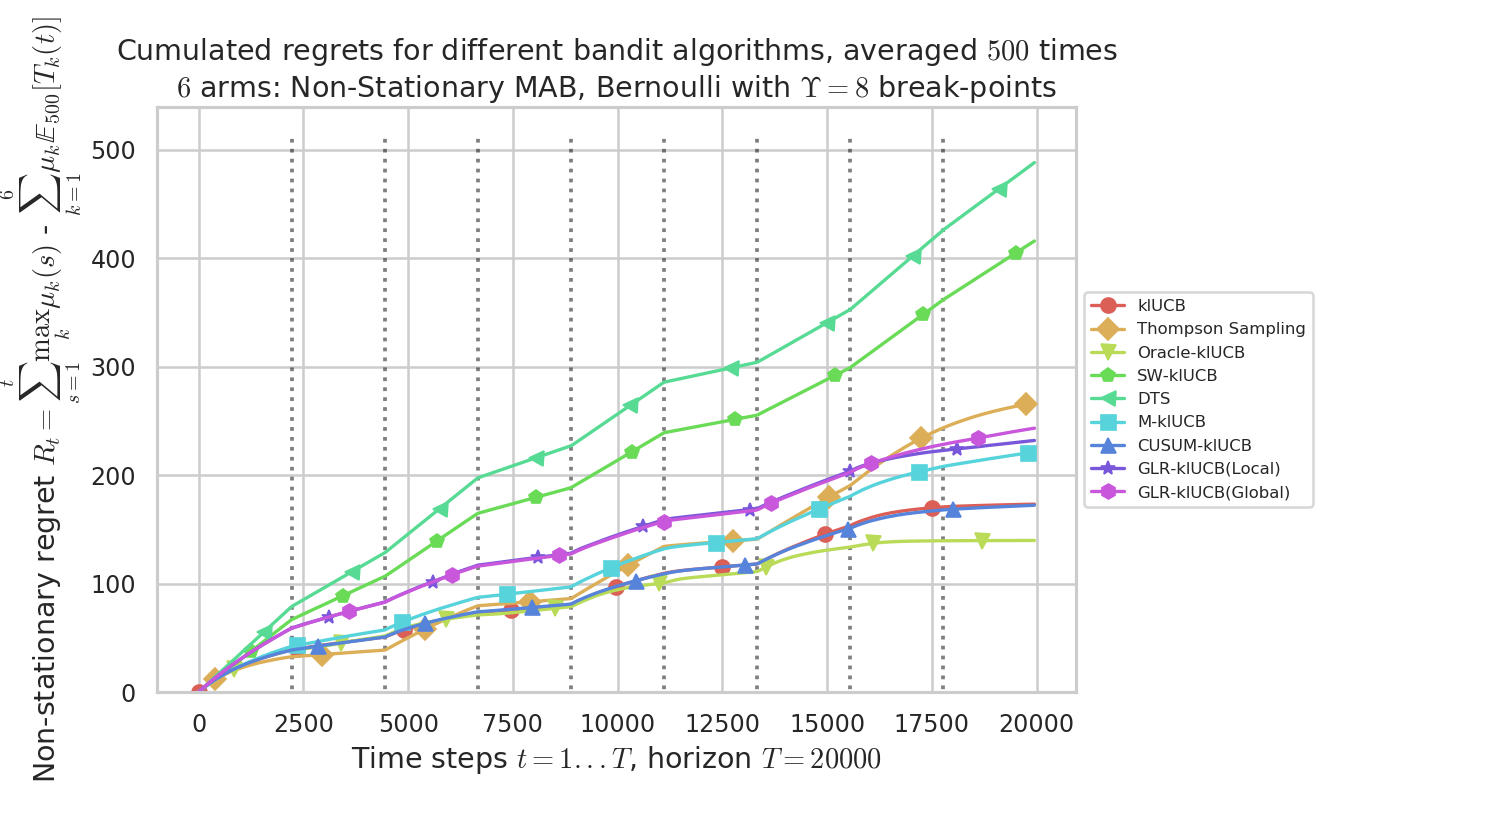
\includegraphics[width=1.09\linewidth]{2-Chapters/6-Chapter/nonstatbandits.git/figures/SP__K6_T20000_N500__9_algos_pb3/main____env1-1_8638317743626238996.pdf}
    \caption{Mean regret as a function of time, $R_t$ ($1 \leq t \leq T = 20000$) for problem 3.}
    \label{fig:6:meanRegretPb3}
\end{figure}


% -----------------------------------------------------------------
\begin{figure}[h!]  % [htbp]
    \centering
    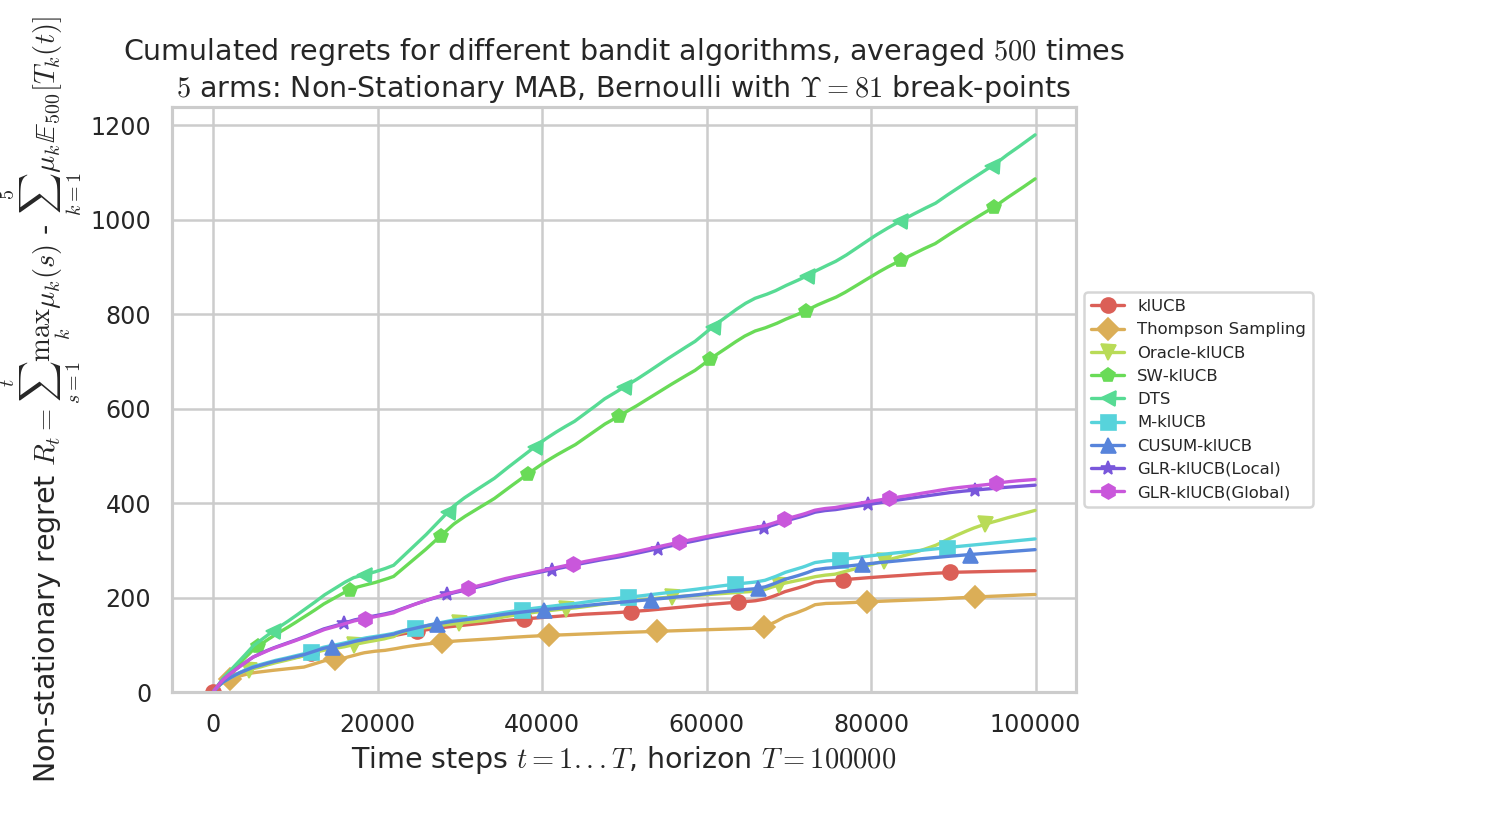
\includegraphics[width=1.09\linewidth]{2-Chapters/6-Chapter/nonstatbandits.git/figures/SP__K5_T100000_N500__9_algos_pb5/main____env1-1_950848333706043320.pdf}
    \caption{Mean regret as a function of time, $R_t$ ($1 \leq t \leq T = 100000$) for problem 5.}
    \label{fig:6:meanRegretPb5}
\end{figure}


% ----------------------------------------------------------------------------
% ----------------------------------------------------------------------------
\subsection{Omitted proofs}\label{proof:6:Conc}
% ----------------------------------------------------------------------------

This Appendix gives some proofs omitted in the main text of this chapter.
Missing proofs can be found in the article \cite{Besson2019GLRT}.

% ----------------------------------------------------------------------------
\subsubsection{Pinsker's inequality}\label{proof:6:Pinsker}

Pinsker's inequality is proved below, using simple real analysis arguments\footnote{~The proof is inspired by Lemma~10.2 from \cite{LattimoreBanditAlgorithmsBook} (version $1699$ of January $2019$).}.

\begin{lemma}[Pinsker's inequality]\label{lem:6:Pinsker}
    Let $p,q\in[0,1]$, and $\kl(p,q) = p \ln\left(\frac{p}{q}\right) + (1-p)\ln\left(\frac{1-p}{1-q}\right)$.
    Then $\kl(p,q) \geq 2 (p-q)^2$.
\end{lemma}
\begin{proof}
    Fix $p$, and consider the function $g(x) := \kl(p, p+x) - 2 x^2$ ($x$ will be $q-p$), for $x\in(-p, 1-p)$.
    We first observe that $g(0) = 0$, and we easily prove that $x=0$ is the unique minimizer of $g$ over its domain.
    By definition, $\kl$ is of class $\cC^1$ on its two variables, on $(0,1)$, so $g$ is of class $\cC^1$ on the interior of its domain, $(-p, 1-p)$.
    Let us compute its derivative, $g'(x) = (\frac{\partial \; \kl}{\partial 2})(p, p + x) - 4x$.
    Simple calculations yield
    \[ \left(\frac{\partial \; \kl}{\partial 2}\right) (p, p + x) = - \frac{p}{p+x} + \frac{1-p}{1-(p+x)} =  = -x \frac{(2(p + x) - 1)^2}{(p + x)(p + x - 1)}. \]
    % https://www.wolframalpha.com/input/?i=diff(p+*+log(p%2F(p%2Bx))+%2B+(1-p)+*+log((1-p)%2F(1-(p%2Bx)))+-+2*x**2,+x)
    We can verify that $g'(0) = -1 + 1 - 4 \times 0 = 0$, and it has the sign of $-x$ on its domain, as $p + x - 1 < 0$ because $x < 1 - p$, and $p + x > 0$.
    So $g'$ is first positive then negative, so $g$ is increasing then decreasing on its domain, with a change in its monotony at $x=0$, and thus it indeed has a unique minimizer.
    We conclude that $g(x) \geq g(0) = 0$ on $(-p, 1-p)$, and so $\kl(p,q) \geq 2 (p-q)^2$ if $x = q-p$.

    The edge case is the ends of the interval, that is if $x=-p$ or $x=1-p$, that is if $q=0$ or $q=1$.
    If $p\in(0,1)$, then computing the limit of $\kl(p,q)$ for $q\to0^+$ and $q\to1^-$ is obvious and gives $\kl(p,q) \to +\infty$, while the right-hand side of Pinsker's inequality stays finite (so the inequality is still true at the limit).
    If $p=0$ or $p=1$, the same computation works, by the convention that $p \log(p) = 0$ if $p=0$.
    %
    % Bonus: one can verify our computation in Python with the SymPy module:
    % \begin{verbatim}
    %     $ (bash) python
    %     >>> from sympy import *
    %     >>> x, p = symbols('x p')
    %     >>> g = p * log(p/(p+x)) + (1-p) * log((1-p)/(1-(p+x))) - 2*x**2
    %     >>> print(diff(g, x))
    %     -p/(p + x) - 4*x + (-p + 1)/(-p - x + 1)
    % \end{verbatim}
\end{proof}



% % ----------------------------------------------------------------------------
% \subsubsection{Simplified expression for the GLR statistic}\label{app:6:GLR_with_kl}

% % Remember that the Generalized Likelihood Ratio statistic for the test presented in \eqref{eq:6:firstDefGLRT} in Section~\ref{sub:6:presentationOfGLRTest} is
% % \[\GLR(n) := \frac{\sup\limits_{\mu_0,\mu_1,\tau < n}\ell(X_1, \ldots, X_n ; \mu_0,\mu_1,\tau)}{\sup\limits_{\mu_0}\ell(X_1, \ldots, X_n ; \mu_0)},\]
% % %
% % where $\ell(X_1, \ldots, X_n ; \mu_0)$ and $\ell(X_1, \ldots, X_n ; \mu_0,\mu_1,\tau)$ respectively denote the likelihoods of the first $n$ observations under a model in $\cH_0$ and $\cH_1$.

% The Generalized Likelihood Ratio statistic for the test is presented above in \eqref{eq:6:firstDefGLRT} in Section~\ref{sub:6:presentationOfGLRTest}.
% %
% We refer to \cite{Basseville93} and reference therein for the generic proof, but we prove here the specific case of Bernoulli distributions.
% % For any $k \leq k'$, we denote $\widehat{\mu}_{k:k'} := \frac{1}{k - k' + 1} \sum_{l=k}^{k'} X_l$ denotes the average of the observations $X_l$ collected between the instants $k$ and $k'$.
% %
% We prove below that the GLR test is equivalent to
% \begin{align*}
%     \GLR(n)
%     &= \frac{\sup\limits_{\mu_0,\mu_1,\tau < n}\ell(X_1, \ldots, X_n ; \mu_0,\mu_1,\tau)}{\sup\limits_{\mu_0}\ell(X_1, \ldots, X_n ; \mu_0)} \\
%     &= \exp\Bigl[ \sup_{s \in [2,n-1]} \left[s \times \kl\left(\widehat{\mu}_{1:s},\widehat{\mu}_{1:n}\right) + (n-s) \times \kl\left(\widehat{\mu}_{s+1:n},\widehat{\mu}_{1:n}\right)\right] \Bigr].
% \end{align*}
% %
% % Remember that the binary relative entropy $\kl$, defined for $x,y\in[0,1]$
% % by $\kl(x,y) := x \ln\left(\frac{x}{y}\right) + (1-x)\ln\left(\frac{1-x}{1-y}\right)$,
% % with the usual convention that $t \log(t) = 0$ if $t=0$.

% \begin{proof}
%     First, we consider the denominator in the expression of $\GLR(n)$ \eqref{eq:6:firstDefGLRT}, that is the $\sup$ on $\mu_0$.
%     We have $\ell(X_1, \ldots, X_n ; \mu_0) = \prod_{i=1}^n \ell(X_i ; \mu_0)$ by independence of the observations $X_i$,
%     and $\ell(X_i ; \mu_0) = \mu_0^{X_i} (1-\mu_0)^{1-X_i}$ for Bernoulli distributions.
%     Therefore, taking the logarithm gives
%     \begin{align*}
%         \log\ell(X_1, \ldots, X_n ; \mu_0)
%         &= \sum_{i=1}^n X_i \log(\mu_0) + (1-X_i) \log(1-\mu_0) \\
%         &= \log(\mu_0) \times \left( \sum_{i=1}^n X_i \right) + \log(1-\mu_0) \times \left( n - \sum_{i=1}^n X_i \right) \\
%         &= n \left[ \widehat{\mu}_{1:n} \log(\mu_0) + (1 - \widehat{\mu}_{1:n}) \log(1-\mu_0) \right].
%     \end{align*}
%     %
%     For a constant $a\in[0,1]$, let $h(x) := a \log(x) + (1-a) \log(1-x)$ on $(0,1)$,
%     and we are trying to solve $\sup_{x\in[0,1]} h(x)$.
%     If $a=0$ or $a=1$, $h$ is maximum at $x=a$.
%     Now if $a\neq0$, As $h$ is of class $\cC^1$, we can just differentiate and find the root of its derivative:
%     $h'(x) = a/x - (1-a)/(1-x)$, so $h'(x) = 0$ if and only if $x=a$.
%     Thus in all cases, $\sup_{x\in[0,1]} h(x) = h(a)$.
%     %
%     Here, we have $a = \widehat{\mu}_{1:n}$, and thus we solve the $\sup_{\mu_0}$ optimization problem found in the denominator of the $\GLR(n)$ expression.
%     By replacing $\mu_0 = \widehat{\mu}_{1:n}$, we obtained the following (unique) solution,
%     \begin{equation}\label{eq:6:solutionPbOpt_for_1n}
%         \sup_{\mu_0} \log\ell(X_1, \ldots, X_n ; \mu_0) = n \left( \widehat{\mu}_{1:n} \log(\widehat{\mu}_{1:n}) + (1 - \widehat{\mu}_{1:n}) \log(1-\widehat{\mu}_{1:n}) \right).
%     \end{equation}

%     Now let us consider the nominator of the $\GLR(n)$ expression.
%     We can again work with log-likelihoods, and so we have
%     \begin{align*}
%         \log\ell(X_1, \ldots, X_n ; \mu_0,\mu_1,\tau)
%         &= \sum_{i=1}^{\tau} X_i \log(\mu_0) + (1-X_i) \log(1-\mu_0) + \sum_{i=\tau+1}^n X_i \log(\mu_1) + (1-X_i) \log(1-\mu_1) \\
%         &= s \bigl( \widehat{\mu}_{1:s} \log(\mu_0) + (1 - \widehat{\mu}_{1:s}) \log(1-\mu_0) \bigr) \\
%         & \;\;\;\; + (n-s) \bigl( \widehat{\mu}_{s+1:n} \log(\mu_1) + (1 - \widehat{\mu}_{s+1:n}) \log(1-\mu_1) \bigr).
%     \end{align*}
%     Because we solved in \eqref{eq:6:solutionPbOpt_for_1n} the $\sup$ for the denominator,
%     we have
%     \begin{align*}
%         \GLR(n)
%         % &= \frac{\sup\limits_{\mu_0,\mu_1,\tau < n}\ell(X_1, \ldots, X_n ; \mu_0,\mu_1,\tau)}{\sup\limits_{\mu_0}\ell(X_1, \ldots, X_n ; \mu_0)}, \\
%         &= \frac{\sup\limits_{\mu_0,\mu_1,\tau < n}\ell(X_1, \ldots, X_n ; \mu_0,\mu_1,\tau)}{ \exp\left[ n \left( \widehat{\mu}_{1:n} \log(\mu_0) + (1 - \widehat{\mu}_{1:n}) \log(1-\mu_0) \right) \right] }, \\
%         &= \sup\limits_{\mu_0,\mu_1,\tau < n} \frac{\ell(X_1, \ldots, X_n ; \mu_0,\mu_1,\tau)}{ \exp\left[ n \left( \widehat{\mu}_{1:n} \log(\widehat{\mu}_{1:n}) + (1 - \widehat{\mu}_{1:n}) \log(1-\widehat{\mu}_{1:n}) \right) \right] }, \\
%         &= \exp \Bigl[ \sup\limits_{\mu_0,\mu_1,\tau < n} \Bigl[ \log\Bigl[ \frac{\ell(X_1, \ldots, X_n ; \mu_0,\mu_1,\tau)}{ \exp\left[ n \left( \widehat{\mu}_{1:n} \log(\widehat{\mu}_{1:n}) + (1 - \widehat{\mu}_{1:n}) \log(1-\widehat{\mu}_{1:n}) \right) \right] } \Bigr] \Bigr] \Bigr],  \\
%         &= \exp \Bigl[ \sup\limits_{\mu_0,\mu_1, 1 < s < n} \Bigl[
%             s \bigl( \widehat{\mu}_{1:s} \log(\mu_0) + (1 - \widehat{\mu}_{1:s}) \log(1-\mu_0) \bigr) \\
%             & \hspace{35pt} + (n-s) \bigl( \widehat{\mu}_{s+1:n} \log(\mu_1) + (1 - \widehat{\mu}_{s+1:n}) \log(1-\mu_1) \bigr) \\
%             & \hspace{35pt} - n \bigl( \widehat{\mu}_{1:n} \log(\widehat{\mu}_{1:n}) + (1 - \widehat{\mu}_{1:n}) \log(1-\widehat{\mu}_{1:n}) \bigr)
%         \Bigr] \Bigr].
%     \end{align*}
%     By linearity and independence, we can separate the joint optimization problem on $\mu_0,\mu_1,s$ in two optimizations problems for $\mu_0,s$ and $\mu_1,s$, that can first be solved explicitly for $\mu_0$ (resp. $\mu_1$) and then left to be solved for $s$.
%     By definition, $n \; \widehat{\mu}_{1:n} = \sum_{i=1}^n X_i = s \;\widehat{\mu}_{1:s} + (n-s) \;\widehat{\mu}_{s+1:n}$, so the right hand side (negative) part involving $\widehat{\mu}_{1:n}$ can be distributed in the two left hand side (positive) terms,
%     which are both handled similarly.
%     For instance for $\mu_0$, we use the same computation as above with the function $h$ to find the optimum:
%     $\widehat{\mu}_{1:s} \log(\mu_0) + (1 - \widehat{\mu}_{1:s}) \log(1-\mu_0)$
%     is optimum for $\mu_0 = \widehat{\mu}_{1:s}$.
%     Similarly, the term for $\mu_1$ gives that $\sup_{\mu_1} \widehat{\mu}_{s+1:n} \log(\mu_1) + (1 - \widehat{\mu}_{s+1:n}) \log(1-\mu_1)$
%     is attained for $\mu_1 = \widehat{\mu}_{s+1:n}$.
%     Finally, by replacing the two expressions of the solutions for $\mu_0$ and $\mu_1$,
%     we obtain
%     \begin{align*}
%         \GLR(n)
%         = \exp \Bigl[ \sup\limits_{1 < s < n} \Bigl[
%             s \times \Bigl(
%                     & \widehat{\mu}_{1:s} \log(\widehat{\mu}_{1:s}) + (1 - \widehat{\mu}_{1:s}) \log(1-\widehat{\mu}_{1:s}) \\
%                     & - \widehat{\mu}_{1:s} \log(\widehat{\mu}_{1:n}) + (1 - \widehat{\mu}_{1:s}) \log(1-\widehat{\mu}_{1:n})
%             \Bigr) \\
%             + (n-s) \times \Bigl(
%                 & \widehat{\mu}_{s+1:n} \log(\widehat{\mu}_{s+1:n}) + (1 - \widehat{\mu}_{s+1:n}) \log(1-\widehat{\mu}_{s+1:n}) \\
%                 & - \widehat{\mu}_{s+1:n} \log(\widehat{\mu}_{1:n}) + (1 - \widehat{\mu}_{s+1:n}) \log(1-\widehat{\mu}_{1:n})
%             \Bigr)
%         \Bigr] \Bigr].
%     \end{align*}
%     We conclude by recognizing the expressions of $s \times \kl(\widehat{\mu}_{1:s}, \widehat{\mu}_{1:n})$
%     and $(n-s) \times \kl(\widehat{\mu}_{s+1:n}, \widehat{\mu}_{1:n})$.
% \end{proof}


% Consider $(Y_i)_{i\in\N}$ some data, and $t_0\in\N$, $t\in\N$ and any $s\in[t_0,t)$.
% For any $a<b$, define $\mu_{a:b} := \frac{1}{b-a+1} \sum_{i=a}^{b} Y_i$ the mean of samples from $a$ to $b$.

% In a one dimensional exponential family, \eg, Gaussian distributions of known variance ($\sigma=1$) or Bernoulli distributions, the Kullback-Leibler divergence of two distributions is expressed with a $\kl$ function of their mean.
% That is, for two distributions $\nu_1,\nu_2$ of means $\mu_1,\mu_2$,
% $$\KL(\nu_1,\nu_2) = \kl(\mu_1,\mu_2).$$

% The \GLR{} test is defined in \cite{Maillard2018GLR}, and is written like this.
% $$\GLR^{\kl}_{t_0 : s : t} = (s-t_0+1) \kl(\mu_{t_0:s}, \mu_{t_0:t}) + (t-s) \kl(\mu_{s+1:t}, \mu_{t_0:t}).$$

% \begin{lemma}[Simplified expression for $\GaussianGLR$]\label{lem:XXX}
%     For $\cN_1$, the exponential family of Gaussian distributions of variance $\sigma^2=1$,
%     the \GLR{} test can be simplified:
%     \begin{align}
%         \forall t_0 \leq s < t,\; \GaussianGLR_{t_0 : s : t} &= (s-t_0+1) \kl(\mu_{t_0:s}, \mu_{t_0:t}) + (t-s) \kl(\mu_{s+1:t}, \mu_{t_0:t})\\
%         &= \frac{(s-t_0+1)(t-s)}{t-t_0+1} \kl(\mu_{s+1:t}, \mu_{t_0:s}) = \frac{(s-t_0+1)(t-s)}{t-t_0+1} \frac{(\mu_{s+1:t}, \mu_{t_0:s})^2}{2}.
%     \end{align}
% \end{lemma}
% \begin{proof}
%     Define $k_1 := \kl(\mu_{t_0:s}, \mu_{t_0:t})$,
%     $k_2 := \kl(\mu_{s+1:t}, \mu_{t_0:t})$,
%     and $k_3 := \kl(\mu_{s+1:t}, \mu_{t_0:s})$.
%     In this family $\cN_1$, $\kl(x,y) = \frac{(x-y)^2}{2}$. Let us multiply everything by $2$ to avoid having this $\frac{1}{2}$ on every line.
%     % \begin{small}
%     \begin{align*}
%         &2 (s-t_0+1) k_1 + (t-s) k_2 \\
%         &=
%         (s-t_0+1)\mu_{t_0:s}^2 + (t-s)\mu_{s+1:t}^2 + (s-t_0+1+t-s)\mu_{t_0:t}^2 \\
%         &\;\;\;\;\;\;\;\;\;- 2 (s-t_0+1)\mu_{t_0:s}\mu_{t_0:t}
%         - 2 (t-s)\mu_{s+1:t}\mu_{t_0:t} \\
%         &= (s-t_0+1)\mu_{t_0:s}^2 + (t-s)\mu_{s+1:t}^2 + (t-t_0+1)\mu_{t_0:t}^2 \\
%         &\;\;\;\;\;\;\;\;\;- 2 (\underbrace{(s-t_0+1)\mu_{t_0:s}+(t-s)\mu_{s+1:t}}_{=\sum_{i=t_0}^{t} Y_i = (t-t_0+1) \mu_{t_0:t}})\mu_{t_0:t} \\
%         &= (s-t_0+1)\mu_{t_0:s}^2 + (t-s)\mu_{s+1:t}^2 - (t-t_0+1)\mu_{t_0:t}^2 \\
%         &= \frac{\left(\sum_{i=t_0}^{s} Y_i \right)^2}{s-t_0+1} + \frac{\left(\sum_{i=s+1}^{t} Y_i \right)^2}{t-s} - \frac{\left(\sum_{i=t_0}^{t} Y_i \right)^2}{t-t_0+1} \\
%         &= \frac{1}{t-t_0+1} \Bigl( \frac{(s-t_0+1) + (t-s)}{s-t_0+1} \left(\sum_{i=t_0}^{s} Y_i \right)^2 + \frac{(s-t_0+1) + (t-s)}{t-s} \left(\sum_{i=s+1}^{t} Y_i \right)^2 \\
%         &\;\;\;\;\;\;\;\;\;- \left(\sum_{i=t_0}^{s} Y_i + \sum_{i=s+i}^{t} Y_i \right)^2 \Bigr) \\
%         &= \frac{1}{t-t_0+1} \Bigl( \left(\sum_{i=t_0}^{s} Y_i \right)^2 + \frac{t-s}{s-t_0+1} \left(\sum_{i=t_0}^{s} Y_i \right)^2 + \left(\sum_{i=s+1}^{t} Y_i \right)^2 + \frac{s-t_0+1}{t-s} \left(\sum_{i=s+1}^{t} Y_i \right)^2 \\
%         &\;\;\;\;\;\;\;\;- \left(\sum_{i=t_0}^{s} Y_i \right)^2 - \left(\sum_{i=s+i}^{t} Y_i \right)^2 - 2 \left(\sum_{i=t_0}^{s} Y_i \right) \left(\sum_{i=s+i}^{t} Y_i \right) \Bigr) \\
%         &= \frac{1}{t-t_0+1} \Bigl(\frac{t-s}{s-t_0+1} \left(\sum_{i=t_0}^{s} Y_i \right)^2 + \frac{s-t_0+1}{t-s} \left(\sum_{i=s+1}^{t} Y_i \right)^2 - 2 \left(\sum_{i=t_0}^{s} Y_i \right) \left(\sum_{i=s+i}^{t} Y_i \right) \Bigr) \\
%         &= \frac{(s-t_0+1)(t-s)}{t-t_0+1} \Bigl( \frac{1}{(s-t_0+1)^2} \left(\sum_{i=t_0}^{s} Y_i \right)^2 + \frac{1}{(t-s)^2} \left(\sum_{i=s+1}^{t} Y_i \right)^2 \\
%         &\;\;\;\;\;\;\;\;\;- 2 \left(\frac{1}{s-t_0+1} \sum_{i=t_0}^{s} Y_i \right) \left(\frac{1}{t-s} \sum_{i=s+1}^{t} Y_i \right) \Bigr) \\
%         &= \frac{(s-t_0+1)(t-s)}{t-t_0+1} (\mu_{s+1:t} - \mu_{t_0:s})^2 = 2 \frac{(s-t_0+1)(t-s)}{t-t_0+1} k_3.
%     \end{align*}
%     as wanted.
%     % \end{small}
% \end{proof}

% This is not true for all one dimensional exponential family, for instance for Bernoulli distributions it is almost never the case.
% Imagine $t_0=0, t=2, s=1$ and data $Y_i = [0,1]$.
% Then $\mu_{t_0:s}=0$, $\mu_{s+1:t}=1$, $\mu_{t_0:t}=0.5$, and so $k_1 = \kl(0,0.5) = \log(2)$ and $k_2 = \kl(1,0.5)=\log(2)$ and $k_3=\kl(0,1)=-\infty$ so we do not have
% $(s-t_0+1) \kl(\mu_{t_0:s}, \mu_{t_0:t}) + (t-s) \kl(\mu_{s+1:t}, \mu_{t_0:t}) = \frac{(s-t_0+1)(t-s)}{t-t_0+1} \kl(\mu_{s+1:t}, \mu_{t_0:s})$.



% ----------------------------------------------------------------------------
\subsubsection{Proof of Lemma~\ref{lem:6:ConcFirst}.}
\label{app:6:proofConcFirst}
%
Using the same construction as in the proof of Theorem~14 in \cite{KK18Martingales}, one can prove that for every $\lambda \in I$ (for an interval $I$), there exists a non-negative super-martingale $M^\lambda (s)$ with respect to the filtration $\cF_t = \sigma(X_1,\dots,X_t)$ that satisfies $\bE[M^\lambda(s)] \leq 1$ and
\[\forall s \in \N^*, \ \ M^\lambda (s) \geq \mathrm{e}^{\lambda [s \, \kl(\widehat{\mu}_s,\mu) - 3\ln(1+\ln(s))] - g(\lambda)}\]
for some function $g : I \rightarrow \R$. This super-martingale is of the form
$M^\lambda (s) = \int \mathrm{e}^{\eta\sum_{i=1}^s X_i - \phi_\mu(\lambda)s} d\pi(\eta)$,
for a well-chosen probability distribution $\pi$, and the function $g$ can be chosen to be any
\begin{eqnarray*}
    g_{\xi} : \left[0; 1/(1+\xi)\right] & \longrightarrow & \R \\
    \lambda & \mapsto & \lambda(1+\xi) \ln \left(\frac{\pi^2}{3(\ln(1+\xi))^2}\right) -  \ln(1 - \lambda(1 + \xi))
\end{eqnarray*}
for a parameter $\xi \in [0,1/2]$.

Similarly, there exists an independent super-martingale $W^\lambda (r)$ w.r.t. the filtration $\cF_r' = \sigma(Y_1,\dots,Y_r)$ such that
\[\forall r \in \N^*, \ \ W^\lambda (r) \geq \mathrm{e}^{\lambda [r\kl(\widehat{\mu}'_r,\mu) - 3\ln(1+\ln(r))] - g(\lambda)},\]
for the same function $g(\lambda)$.
In the terminology of \cite{KK18Martingales}, the processes $\bm{X}(s) = s \, \kl(\widehat{\mu}_s,\mu) - 3\ln(1+\ln(s))$ and $\bm{Y}(s) = r \, \kl(\widehat{\mu}_r,\mu) - 3\ln(1+\ln(r))$ are called $g$-DCC for Doob-Cram\'er-Chernoff, as Doob's inequality can be applied in combination with the Cram\'er-Chernoff method to obtain deviation inequalities that are uniform in time.

Here we have to modify the technique used in their Lemma 4 in order to take into account the two stochastic processes, and the presence of super-martingales instead of martingales (for which Doob inequality still works).
One can write
%
\begin{align*}
    &\bP\bigl( \exists r \in \N^* : s \, \kl\left(\widehat{\mu}_{s},\mu\right) + r \, \kl\left(\widehat{\mu}_r',\mu'\right) > 3\ln(1+\ln(s)) + 3\ln(1+\ln(r)) + u \bigr) \\
    & \leq \bP\left(\exists r \in \N^* : M^\lambda(s)W^\lambda(r) > \mathrm{e}^{\lambda u - 2g(\lambda)}\right) \\
    & = \lim_{n \rightarrow \infty} \bP\left(\exists r \in [n] :  M^\lambda(s)W^\lambda(r) > \mathrm{e}^{\lambda u - 2g(\lambda)}\right) \\
    & = \lim_{n \rightarrow \infty} \bP\left(\sup_{r \in [n]}  M^\lambda(s)W^\lambda(r) > \mathrm{e}^{\lambda u - 2g(\lambda)}\right).
\end{align*}
%
Using that $\tilde{M}(r) = M^\lambda(s)W^\lambda(r)$ is a super-martingale with respect to the filtration $\tilde{\cF}_r = \sigma(X_1,\dots,X_s, Y_1,\dots,Y_r)$, one can apply Doob's maximal inequality to obtain
\begin{eqnarray*}
    \bP\left(\sup_{r \in [n]}  M^\lambda(s)W^\lambda(r) > \mathrm{e}^{\lambda u - 2g(\lambda)}\right) &\leq& \mathrm{e}^{-(\lambda u - 2g(\lambda))}\bE[\tilde{M}(1))] \\
    & = & \mathrm{e}^{-(\lambda u - 2g(\lambda))}\bE[M^\lambda(s)W^\lambda(1)] \\
    & \leq & \mathrm{e}^{-(\lambda u - 2g(\lambda))},
\end{eqnarray*}
using that $M^\lambda(s)$ and $W^\lambda(1)$ are independent and have an expectation smaller than $1$.

Putting things together yields
\[\bP\left(\exists r \in \N^* : s \, \kl\left(\widehat{\mu}_{s},\mu\right) + r \, \kl\left(\widehat{\mu}_r',\mu'\right) > 3\ln(1+\ln(s)) + 3\ln(1+\ln(r)) + u\right) \leq \mathrm{e}^{-\left(\lambda u - 2g_{\xi}(\lambda)\right)},\]
for any function $g_{\xi}$ defined above.
%
The conclusion follows by optimizing for both $\lambda$ and $\xi$, using Lemma~18 in \cite{KK18Martingales}.


% ----------------------------------------------------------------------------
\subsubsection{A Concentration Result Involving Two Arms}\label{proof:6:Chernoff2arms}

The following result is useful to control the probability of the good event in our two regret analyzes.
Its proof follows from a straightforward application of the Cram\'er-Chernoff method \cite{Boucheron2013}, and is given below.

\begin{lemma}\label{lem:6:Chernoff2arms}
    Let $\widehat{\mu}_{i,s}$ be the empirical mean of $s$ \iid{} observations with mean $\mu_i$, for $i \in \{a,b\}$, that are $\sigma^2$-sub-Gaussian. Define $\Delta = \mu_a - \mu_b$. Then for any $s,r > 0$, we have
    \begin{equation}
        \bP\left(\frac{s \; r}{s+r}\Big(\widehat{\mu}_{a,s} - \widehat{\mu}_{b,r} - \Delta\Big)^2 \geq u \right) \leq 2\exp\left(- \frac{u}{2\sigma^2}\right).
    \end{equation}
\end{lemma}


\paragraph{Proof of Lemma~\ref{lem:6:Chernoff2arms}.}

We first note that
\begin{align}\label{eq:6:Preparation}
	&\bP\left(\frac{s \; r}{s+r}\Big(\widehat{\mu}_{a,s} - \widehat{\mu}_{b,r} - \Delta\Big)^2 \geq u \right) \nonumber\\
	&\leq \bP\left(\widehat{\mu}_{a,s} - \widehat{\mu}_{b,r} \geq \Delta + \sqrt{\frac{s+r}{sr}u} \right) + \bP\left(\widehat{\mu}_{b,r} - \widehat{\mu}_{a,s} \geq -\Delta + \sqrt{\frac{s+r}{sr}u} \right),
\end{align}
and those two quantities can be upper-bounded similarly using the Cram\'er-Chernoff method.

Let $(X_i)$ and $(Y_i)$ be two \iid{} sequences that are $\sigma^2$ sub-Gaussian with mean $\mu_1$ and $\mu_2$ respectively. Let $n_1$ and $n_2$ be two integers and $\widehat{\mu}_{1,n_1}$ and $\widehat{\mu}_{2,n_2}$ denote the two empirical means based on $n_1$ observations from $X_i$, and $n_2$ observations from $Y_i$ respectively.
Then for every $\lambda > 0$, we have
\begin{eqnarray*}
    \bP\left(\widehat{\mu}_{1,n_1} - \widehat{\mu}_{2,n_2} \geq \mu_1 - \mu_2 + x \right)
    & \leq & \bP\left(\frac{1}{n_1}\sum_{i=1}^{n_1} (X_i-\mu_1) - \frac{1}{n_2}\sum_{i=1}^{n_2} (Y_i - \mu_2) \geq x \right)\\
    & \leq & \bP\left(\mathrm{e}^{\lambda \left(\frac{1}{n_1}\sum\limits_{i=1}^{n_1} (X_i-\mu_1) - \frac{1}{n_2}\sum\limits_{i=1}^{n_2} (Y_i - \mu_2)\right)} \geq \mathrm{e}^{\lambda x} \right)
\end{eqnarray*}
And so thanks to Markov's inequality, we obtain
\begin{eqnarray*}
    \bP\left(\widehat{\mu}_{1,n_1} - \widehat{\mu}_{2,n_2} \geq \mu_1 - \mu_2 + x \right)
    & \leq & \mathrm{e}^{-\lambda x}\bE\left[\mathrm{e}^{\lambda \frac{1}{n_1}\sum\limits_{i=1}^{n_1} (X_i-\mu_1)}\right]\bE\left[\mathrm{e}^{-\lambda \frac{1}{n_2}\sum\limits_{i=1}^{n_2} (Y_i-\mu_2)}\right] \\
    & = & \exp\left(- \lambda x + n_1\phi_{X_1 - \mu_1}\left(\frac{\lambda}{n_1}\right) + n_2\phi_{Y_1 - \mu_2}\left(-\frac{\lambda}{n_2}\right)\right) \\
    & \leq & \exp\left(- \lambda x + \frac{\lambda^2\sigma^2}{2n_2} + \frac{\lambda^2\sigma^2}{2n_1}\right),
\end{eqnarray*}
%
where the last inequality uses the sub-Gaussian property.
%
Choosing the value
\[\lambda = \frac{x}{2\left[\sigma^2/(2n_1) + \sigma^2/(2n_2)\right]}\]
which minimizes the right-hand side of the inequality yields
\[\bP\left(\widehat{\mu}_{1,n_1} - \widehat{\mu}_{2,n_2} \geq \mu_1 - \mu_2 + x \right) \leq \exp\left(- \frac{n_1n_2}{n_1+n_2}\frac{x^2}{2\sigma^2}\right).\]
%
Using this inequality twice in the right hand side of \eqref{eq:6:Preparation} concludes the proof.
\hfill{} $\qed$  % WARNING manually write this is a bad idea!

% -----------------------------------------------------------------

% -----------------------------------------------------------------
% ------------------------------------------------------------------------------------
% \subsection{Proof for \GLRklUCB{} with Local Changes}
% \label{proof:6:mainRegretBound}

% \TODOL{Si on veut gagner de la place, et éviter les redites, on peut dire que la preuve ressemble à celle pour Global changes, et qu'elle est traitée en annexe de \cite{Besson2019GLRT} de toute façon !}

% % \subsubsection{Proof of Theorem~\ref{thm:6:mainRegretBound}}

% Our analysis for the other variant of \GLRklUCB{} also relies on the general regret decomposition~\eqref{eq:6:GeneRegretBound} and follows the proof skeleton presented in Section~\ref{sub:6:proofSkeleton}, with the following appropriate ``good event'', that is shown to be likely in Lemma~\ref{lem:6:GoodEvent} below.
% %
% \begin{equation}\label{def:6:GoodEvenLocal}
%     \cE_T(\alpha,\delta) = \left(\forall i \in \{1, \ldots, K\}, \forall \ell \in \{1, \ldots, \NCi\}, \hat{\tau}^{(\ell)}_i \in \left[\tau_i^{(\ell)} + 1, \tau_i^{(\ell)} + d_i^{(\ell)}\right] \right),
% \end{equation}
% where $\widehat{\tau}_i^{(\ell)}$ is defined as the $\ell$-th change detected by the algorithm on arm $i$ and $d_i^{(\ell)}=d_i^{(\ell)}(\alpha,\delta)$ is defined as in Assumption~\ref{ass:6:LongPeriods}. Using this assumption, one can prove the following.

% \begin{lemma}\label{lem:6:GoodEvent}
%     The ``bad event'' is highly unlikely, as it satisfies $\bP((\cE_T(\alpha,\delta))^c) \leq 2 \; \delta \; \EffChange$.
% \end{lemma}


% We now turn our attention to upper bounding terms $(A)$ and $(B)$ in \eqref{eq:6:GeneRegretBound}.

% \paragraph{Upper bound on term $\bm{(A)}$.}
% %
% \begin{align*}
%     (A) & \leq \bE\left[\indic(\cE_T) \sum_{t=1}^T \indic\left(n_{i_t^*}(t) \kl\left(\widehat{\mu}_{i_t^*}(t), \mu_{i_t^*}(t)\right) \geq f(t - \tau_{i_t^*}(t))\right)\right] \\
%     & \leq \sum_{i=1}^K \sum_{k=1}^{\NCi}\bE\left[\indic(\cE_T) \sum_{t=1}^T \indic(i_t^* =i) \indic(\tau_i(t) = \widehat{\tau}_i^{(\ell)})\indic\left(n_{i}(t) \kl\left(\widehat{\mu}_{i}(t), \mu_{i}\right) \geq f(t - \widehat{\tau}_{i}^{(\ell)})\right)\right] \\
%     & \leq \sum_{i=1}^K \sum_{\ell=0}^{\NCi}\bE\left[\indic(\cE_T) \sum_{t=\hat{\tau}_i^{(\ell)}}^{\tau_i^{(\ell+1)}} \indic\left(n_{i}(t) \kl\left(\widehat{\mu}_{i}(t), \mu_{i}\right) \geq f(t - \widehat{\tau}_{i}^{(\ell)})\right) + d_i^{(\ell)}(T)\right] \\
%     & \leq \sum_{i=1}^K \sum_{\ell=0}^{\NCi}d_i^{(\ell+1)}(T) + \sum_{i=1}^K \sum_{\ell=0}^{\NCi}\bE\left[\indic(\cC_i^{(\ell)}) \sum_{t=\hat{\tau}_i^{(\ell)}}^{\tau_i^{(\ell+1)}}\indic\left(n_{i}(t) \kl\left(\widehat{\mu}_{i}(t), \mu_{i}\right) \geq f(t - \widehat{\tau}_{i}^{(\ell)})\right)\right],
% \end{align*}%
% %
% where we introduce the event $\cC_i^{(\ell)}$ that all the changes up to the $\ell$-th have been detected:
% \begin{equation}\cC_i^{(\ell)} = \left\{\forall j \leq \ell, \widehat{\tau}_i^{(j)} \in \left[\tau_i^{(j)} + 1, \tau_i^{(j)} + d_i^{(\ell)} \right] \right\}.\label{def:6:EventCi}\end{equation}
% Clearly, $\cE_T \subseteq \cC_i^{(\ell)}$ and $\cC_i^{(\ell)}$ is $\cF_{\widehat{\tau}_i^{(\ell)}}$-measurable. Observe that conditionally to $\cF_{\widehat{\tau}_i^{(\ell)}}$, when $\indic(\cC_i^{(\ell)})$ holds, $\widehat{\mu}_{i}(t)$ is the average of samples that have all mean $\mu_i^{(\ell)}$. Thus, introducing $\widehat{\mu}_s$ as a sequence of \iid{} random variables with mean $\mu_i^{(\ell)}$, one can write
% \begin{align*}
%     &\bE\left[\left.\indic(\cC_i^{(\ell)}) \sum_{t=\hat{\tau}_i^{(\ell)}}^{\tau_i^{(\ell+1)}} \indic\left(n_{i}(t) \kl\left(\widehat{\mu}_{i}(t), \mu_{i}\right) \geq f(t - \widehat{\tau}_{i}^{(\ell)})\right) \right| \cF_{\widehat{\tau}_i^{(\ell)}}\right]\\
%     & = \indic(\cC_i^{(\ell)}) \sum_{t=\hat{\tau}_i^{(\ell)}}^{\tau_i^{(\ell+1)}} \bE\left[\indic\left(n_{i}(t) \kl\left(\widehat{\mu}_{i}(t), \mu_{i}\right) \geq f(t - \widehat{\tau}_{i}^{(\ell)})\right) \;|\; \cF_{\widehat{\tau}_i^{(\ell)}}\right] \\
% % \end{align*}%
% % \begin{align*}
%     & \leq \indic(\cC_i^{(\ell)}) \sum_{t=1}^{\tau_i^{(\ell+1)} - \hat{\tau}_i^{(\ell)}} \bP\left(\exists s \leq t' : s \times \kl(\widehat{\mu}_{s},\mu_i^{(\ell)}) \geq f(t')\right) \\
%     & \leq \sum_{t=1}^T \frac{1}{t\ln(t)} \leq \ln(\ln(T)),
% \end{align*}%
% %
% where the last but one inequality relies on the concentration inequality given in Lemma 2 of \cite{KLUCBJournal}, and the fact that $f(t) = \ln(t) + 3 \ln(\ln(t))$. Finally, the law of total expectation gives
% \begin{equation}
%     (A) \leq \sum_{i=1}^K \sum_{\ell=0}^{\NCi}\left[d_i^{(\ell+1)}(T) + \ln(\ln(T))\right].
%     \label{eq:6:TermAFinal}
% \end{equation}

% \paragraph{Upper bound on term $\bm{(B)}$.}
% %
% Recall that $\mu^*_{i,\ell}$ is defined from the statement of Theorem~\ref{thm:6:mainRegretBound} as the smallest value that still outperforms arm $i$ on the interval between the $\ell$ and $(\ell+1)$-st change of $i$. We let $\tilde{\mu}_{i,s}^{(\ell)}$ denote the empirical mean of the first $s$ observations of arm $i$ made after time $t=\hat{\tau}_i^{(\ell)}+1$. To upper bound Term B, we introduce a sum over all arms and rewrite the sum in $t$ as a sum of consecutive intervals $[\tau_i^{(\ell)}+1, \tau_i^{(\ell+1)}]$.
% %
% The decomposition follows by using furthermore that on $\cE_T$, we have $\tau_i^{\ell} \leq \hat \tau_i^ \ell \leq \tau_i^{\ell+1}$ for all changes, by Assumption~\ref{ass:6:LongPeriods}.
% %
% \begin{align*}
%     (B) & \leq \sum_{i=1}^K\bE\Big[\indic(\cE_T)\sum_{\ell=1}^{\NCi} \sum_{t=\tau_i^{(\ell)}}^{\tau_i^{(\ell+1)}}\left(\mu_{i^*_t}(t) - \overline{\mu}_{i}^{(\ell)}\right)\indic\left(I_t = i, \UCB_i(t) \geq \mu^*_{i,\ell}\right)\Big] \\
%     & \leq \sum_{i=1}^K\sum_{\ell=1}^{\NCi}\bE\Big[\indic(\cE_T)\hat{\tau}_i^{(\ell)} + \indic(\cE_T) \sum_{t=\widehat{\tau}_i^{(\ell)}+1}^{\tau_i^{(\ell+1)}}\indic\left(I_t = i, \UCB_i(t) \geq \mu^*_{i,\ell}\right)\Big] \\
% %     & \leq \sum_{i=1}^K\sum_{\ell=1}^{\NCi}d_i^{(\ell)}+ \sum_{\ell=1}^{\NCi}\bE\Big[\indic(\cE_T) \sum_{t=\hat{\tau}_i^{(\ell)}+1}^{\tau_i^{(\ell+1)}}\sum_{s=1}^{t-\widehat{\tau}_i^{(\ell)}}\indic\left(I_t = i,n_i(t) = s\right) \indic\left(s \times \kl(\tilde{\mu}_{i,s}^{(\ell)}, \mu^*_{\ell,i}) \leq f(\tau_i^{(\ell+1)} - \widehat{\tau}_i^{(\ell)})\right)\Big] \\
%     & \leq \sum_{i=1}^K\sum_{\ell=1}^{\NCi}d_i^{(\ell)}+ \sum_{i=1}^K\sum_{\ell=1}^{\NCi}\bE\Big[\indic(\cC_i^{(\ell)}) \sum_{s=1}^{n_i(\tau_i^{(\ell+1)})}\indic\left(s \times \kl(\tilde{\mu}_{i,s}^{(\ell)}, \mu^*_{i,\ell}) \leq f(\tau_i^{(\ell+1)} - \tau_i^{(\ell)})\right)\Big].
% \end{align*}%
% %
% The last inequality relies on introducing a sum over $\indic(n_i(t) = s)$ and swapping the sums. Conditionally to $\cF_{\widehat{\tau}_i^{(\ell)}}$, when $\cC_i^{(\ell)}$ holds, for $s \in \{1, \ldots, n_i(\tau_i^{(\ell+1)})\}$, $\tilde{\mu}_{i,s}^{(\ell)}$ is the empirical mean from \iid{} observations of mean $\overline{\mu}_i^{(\ell)}$.
% Therefore, introducing $\widehat{\mu}_s$ as a sequence of \iid{} random variables with mean $\overline{\mu}_i^{(\ell)}$, it follows from the law of total expectation that
% %
% \begin{align*}
%     (B) & \leq \sum_{i=1}^K\sum_{\ell=1}^{\NCi} d_i^{(\ell)}
%     + \sum_{i=1}^K\sum_{\ell=1}^{\NCi} \sum_{s=1}^{\tau_i^{(\ell+1)}-\tau_i^{(\ell)}} \bP\left(s \times \kl(\widehat{\mu}_{s}, \mu^*_{i,\ell}) \leq f(\tau_i^{(\ell+1)} - \tau_i^{(\ell)})\right).
% \end{align*}%
% %
% As $\mu^*_{\ell,i} > \mu_i^{(\ell)}$ by definition, we can use the same analysis as in the proof of Fact~2 in Appendix~A.2 of \cite{KLUCBJournal} to show that
% % \begin{align*}
% %     (B)_i & \leq \sum_{\ell=1}^{\NCi}d_i^{(\ell)}+\sum_{\ell=1}^{\NCi}\left[ \frac{\ln(T) + 3\ln\ln(T)}{\kl(\mu_i^{(\ell)}, \mu^*_{\ell,i})} + \sqrt{\frac{2\pi(\kl'(\mu_i^{(\ell)},\mu^*_{\ell,i}))^2}{(\kl(\mu_i^{(\ell)}, \mu^*_{\ell,i}))^2}}\sqrt{\ln(T) + 3\ln\ln(T)} + 2\left(\frac{\kl'(\mu_i^{(\ell)},\mu^*_{\ell,i})}{\kl(\mu_i^{(\ell)}, \mu^*_{\ell,i})}\right)^2\right].
% % \end{align*}
% \begin{align}\label{eq:6:TermBFinal}
%     (B) & \leq \sum_{i=1}^K\sum_{\ell=1}^{\NCi}d_i^{(\ell)}+\sum_{i=1}^K\sum_{\ell=1}^{\NCi}\left[ \frac{\ln(T) + 3\ln\ln(T)}{\kl(\overline{\mu}_i^{(\ell)},\mu^*_{i,\ell})} + O\left(\sqrt{\log(T)}\right)\right].
% \end{align}
% The result follows by combining the decomposition~\eqref{eq:6:GeneRegretBound} with Lemma~\ref{lem:6:GoodEvent} and the bounds \eqref{eq:6:TermAFinal} and \eqref{eq:6:TermBFinal}.


% \subsubsection{Proof of Lemma~\ref{lem:6:GoodEvent}}\label{proof:6:GoodEvent}

% With the event $\cC_i^{(\ell)}$ defined in \eqref{def:6:EventCi}, a simple union bound yields
% \begin{align*}
%     \bP(\cE_T^c) & \leq \sum\limits_{i=1}^K\sum\limits_{\ell=1}^{\NCi} \underbrace{\bP\left(\widehat{\tau}_i^{(\ell)} \leq \tau_i^{(\ell)} \;|\; \cC_i^{(\ell-1)}\right)}_{(a)} + \sum\limits_{i=1}^K\sum\limits_{\ell=1}^{\NCi} \underbrace{\bP\left(\widehat{\tau}_i^{(\ell)} \geq \tau_i^{(\ell)} + d_i^{(\ell)} \;|\; \cC_i^{(\ell-1)}\right)}_{(b)}.
% \end{align*}

% The final result follows by proving that the terms $(a)$ and $(b)$ are both upper bounded by $\delta$.

% \paragraph{Upper bound on $(a)$: controlling the false alarms.}
% Under the bandit algorithm, the change point detector associated to arm $i$ is based on (possibly much) less than $t - \tau_i(t)$ samples from arm $i$, which makes false alarm even less likely to occur. More precisely, we upper bound term $(a)$ by
% %
% \begin{align*}
%     (a) & \leq \bP\left(\exists s < t \leq n_i(\tau_i^{(\ell)}) : s \times \kl\left(\tilde{\mu}_{i,1:s}^{(\ell-1)},\tilde{\mu}_{i,1:t}^{(\ell-1)}\right) + (t - s) \times \kl\left(\tilde{\mu}_{i,s+1:t}^{(\ell-1)},\tilde{\mu}_{i,1:t}^{(\ell-1)}\right) > \beta(t, \delta) \;|\; \cC_i^{(\ell-1)}\right) \\
%     & \leq \bP\left(\exists s < t : s \times \kl(\widehat{\mu}_{1:s},\mu_i^{(\ell-1)}) + (t - s) \times \kl(\widehat{\mu}_{s+1:t}, \mu_{i}^{(\ell-1)}) > \beta(t, \delta)\right),
% \end{align*}
% with $\hat\mu_{s:s'} = \sum_{r=s}^{s'} Z_{i,r}$ where $Z_{i,r}$ is an \iid{} sequence with mean $\mu_i^{(\ell-1)}$.
% Indeed, conditionally to $\cC_i^{(\ell-1)}$, the $n_i(\tau_i^{(\ell)})$ successive observations of arm $i$ arm starting from $\hat \tau_i^{(\ell)}$ are \iid{} with mean $\mu_i^{(\ell-1)}$.
% Using Lemma~\ref{lem:6:ConcFirst}, term $(a)$ is upper bounded by $\delta$.


% \paragraph{Upper bound on term $(b)$: controlling the delay.}
% %
% Controlling the detection delay on arm $i$ under an adaptive sampling scheme can be tricky. Here we need to leverage the forced exploration (Proposition~\ref{prop:6:EnoughSamples}) to be sure we have enough samples to ensure detection: the effect is that delays will be scaled by the exploration parameter $\alpha$.

% First, it follows from Proposition~\ref{prop:6:EnoughSamples} that there exists $\overline{t} \in \left\{\tau_i^{(\ell)}, \dots, \tau_i^{(\ell)} + d_i^{(\ell)} \right\}$ such that
% $n_i(\overline{t}) - n_i(\tau_i^{(\ell)}) = \overline{r}$ where $\overline{r} = \lfloor \frac{\alpha}{K} d_i^{(\ell)}\rfloor$
% (as the mapping $t\mapsto n_i(t) - n_i(\tau_i^{(\ell)})$ is non-decreasing, is $0$ at $t=\tau_i^{(\ell)}$ and its value at $\tau_i^{(\ell)}+d_i^{(\ell)}$ is larger than $\overline{r}$).
% Using that $(\widehat{\tau}_i^{(\ell)} \geq \tau_i^{(\ell)} + d_i^{(\ell)}) \subseteq (\widehat{\tau}_i^{(\ell)} \geq \overline{t})$,
% the event $(\widehat{\tau}_i^{(\ell)} \geq \tau_i^{(\ell)} + d_i^{(\ell)})$ further implies that
% \[
%     n_i(\tau_i^{(\ell)}) \, \kl\left(\tilde{\mu}^{\ell-1}_{i,n_i(\tau_i^{(\ell)})},\tilde{\mu}^{\ell-1}_{i,n_i(\overline{t})}\right)
%     +  \overline{r} \, \kl\left(\tilde{\mu}^{\ell-1}_{i,n_i(\tau_i^{(\ell)}) : n_i(\overline{t})},\tilde{\mu}^{\ell-1}_{i,n_i(\overline{t})}\right) \leq \beta(n_i(\tau_i^{(\ell)}) + \overline{r},\delta),
% \]
% where $\tilde{\mu}^{\ell-1}_{i,s}$ denotes the empirical mean of the $s$ first observation of arm $i$ since the $(\ell-1)$-th restart $\hat{\tau}_i^{(\ell-1)}$ and  $\tilde{\mu}^{\ell-1}_{i,s:s'}$ the empirical mean that includes observation number $s$ to number $s'$. Conditionally to $\cC^{(\ell-1)}_i$, $\tilde{\mu}^{\ell-1}_{i,n_i(\tau_i^{(\ell)})}$ is the empirical mean of $n_i(\tau_i^{(\ell)})$ \iid{} replications of mean $\mu_i^{\ell-1}$, whereas $\tilde{\mu}^{\ell-1}_{i,n_i(\tau_i^{(\ell)}) : n_i(\overline{t})}$ is the empirical mean of $\overline{r}$ \iid{} replications of mean $\mu_i^{\ell}$.

% Moreover, due to Proposition~\ref{prop:6:EnoughSamples}, $n_i(\tau_i^{(\ell)})$ lies in $
% \left\{\left\lfloor \frac{\alpha}{K}\left(\tau_i^{(\ell)}-\widehat{\tau}_i^{(\ell-1)}\right)\right\rfloor, \dots, \tau_i^{(\ell)}-\widehat{\tau}_i^{(\ell-1)} \right\}$.
% %
% Conditionally to $\cC_i^{(\ell-1)}$, one obtains furthermore using that $d_i^{(\ell-1)} \leq (\tau_i^{(\ell)} - \tau_i^{(\ell-1)})/2$ -- which follows from Assumption~\ref{ass:6:LongPeriods} -- that
% \begin{eqnarray*}
%     n_i(\tau_i^{(\ell)})& \in &  \left\{ \left\lfloor \frac{\alpha}{K}\left(\tau_i^{(\ell)}-\tau_i^{(\ell-1)} - d_i^{(\ell-1)}\right)\right\rfloor, \dots, \left(\tau_i^{(\ell)}-\tau_i^{(\ell-1)}\right) \right\} \\
%     n_i(\tau_i^{(\ell)})& \in& \left\{ \left\lfloor \frac{\alpha}{2K}\left(\tau_i^{(\ell)}-\tau_i^{(\ell-1)}\right)\right\rfloor, \dots, \left(\tau_i^{(\ell)}-\tau_i^{(\ell-1)}\right) \right\} = \cI_k.
% \end{eqnarray*}

% Introducing $\widehat{\mu}_{a,s}$ (resp. $\widehat{\mu}_{b,s}$) the empirical mean of $s$ \iid{} observations with mean $\widehat{\mu}_i^{(\ell-1)}$ (resp. $\widehat{\mu}_i^{(\ell)}$), such that $\widehat{\mu}_{a,s}$ and $\widehat{\mu}_{b,r}$ are independent, it follows that
% \[
%     (b)  \leq \bP\left(\exists s \in \cI_k : s \, \kl\left(\widehat{\mu}_{a,s},\frac{s\widehat{\mu}_{a,s}+\overline{r}\widehat{\mu}_{b,\overline{r}}}{s+\overline{r}} \right) +  \overline{r} \, \kl\left(\widehat{\mu}_{b,\overline{r}},\frac{s\widehat{\mu}_{a,s}+\overline{r}\widehat{\mu}_{b,\overline{r}}}{s+\overline{r}}  \right)  \leq \beta(s+\overline{r},\delta)\right),
% \]
% where we have also used that $\tilde{\mu}^{\ell-1}_{i,n_i(\overline{t})} = \frac{n_i(\tau_i^{(\ell)})\tilde{\mu}^{\ell-1}_{i,n_i(\tau_i^{(\ell)})} + \overline{r}\tilde{\mu}^{\ell-1}_{i,n_i(\tau_i^{(\ell)}) : n_i(\overline{t})}}{n_i(\tau_i^{(\ell)}) + \overline{r}}$.

% Using Pinsker's inequality (Lemma~\ref{lem:6:Pinsker}) and introducing the gap $\Delta_i^{(\ell)} = \mu_i^{(\ell-1)} - {\mu}_i^{(\ell)}$, one can write
% \begin{align}
%     (b) & \leq \bP\left(\exists s \in \cI_k : \frac{2s\overline{r}}{s+\overline{r}}\left(\widehat{\mu}_{a,s} - \widehat{\mu}_{b,\overline{r}} \right)^2  \leq \beta(s+\overline{r},\delta)\right)\nonumber\\
%     & \leq \bP\left(\exists s \in \N : \frac{2sr}{s+r}\left(\widehat{\mu}_{a,s} - \widehat{\mu}_{b,s} - \Delta_i^{(\ell)}\right)^2  \geq \beta(s+r,\delta)\right) \nonumber\\
%     & + \bP\left(\exists s \in \cI_k : \frac{2s\overline{r}}{s+\overline{r}}\left(\widehat{\mu}_{a,s} - \widehat{\mu}_{b,\overline{r}} - \Delta_i^{(\ell)}\right)^2  \leq \beta(s+\overline{r},\delta), \frac{2s\overline{r}}{s+\overline{r}}\left(\widehat{\mu}_{a,s} - \widehat{\mu}_{b,\overline{r}}\right)^2  \leq \beta(s+\overline{r},\delta)\right) \nonumber
% \end{align}
% %

% Using Lemma~\ref{lem:6:Chernoff2arms} stated in Appendix~\ref{proof:6:Chernoff2arms}, and a union bound, the first term in the right hand side is upper bounded by $\delta$ (as $\beta(r+s,\delta) \geq \beta(r,\delta) \geq \log(3s\sqrt{s}/\delta)$). For the second term, we use the observation
% \[\frac{2s \; \overline{r}}{s+\overline{r}}\left(\widehat{\mu}_{a,s} - \widehat{\mu}_{b,\overline{r}} - \Delta_i^{(\ell)}\right)^2  \leq \beta(s+\overline{r},\delta) \ \ \Rightarrow \ \ |\widehat{\mu}_{a,s} - \widehat{\mu}_{b,\overline{r}}| \geq |\Delta_i^{(\ell)}| - \sqrt{\frac{s+\overline{r}}{2\overline{r}s}\beta(s+\overline{r},\delta)}\]
% and finally get
% %
% \begin{equation}\label{eq:6:FromHere}
%     (b) \leq \delta + \bP\left(\exists s \in \cI_k : |\Delta_i^{(\ell)}| \leq 2\sqrt{\frac{s+\overline{r}}{2s\overline{r}}\beta(s+\overline{r},\delta)}\right).
% \end{equation}
% %
% Define $s_{\min} = \left\lfloor \frac{\alpha}{K} (\tau_i^{(\ell)}-\tau_i^{(\ell-1)})/2\right\rfloor$. Using that the mappings $s \mapsto (s+\overline{r})/s\overline{r}$ and $s \mapsto \beta(s + \overline{r},\delta)$ are respectively decreasing and increasing in $s$, one has, for all $s\in \cI_k$,
% \begin{eqnarray*}
%     2\frac{s+\overline{r}}{s \; \overline{r}}\beta\left(s+\overline{r}, \delta\right) & \leq &
%     2\frac{s_{\min}+\overline{r}}{s_{\min} \; \overline{r}}\beta\left(T, \delta\right) \leq \frac{4\beta(T,\delta)}{\left\lfloor \frac{\alpha}{K}d_i^{(\ell)}\right\rfloor},
% \end{eqnarray*}
% %
% where the last inequality follows from the fact that $\overline{r} \leq s_{\min}$ as $d_i^{(\ell)} \leq (\tau_i^{(\ell)} - \tau_i^{(\ell-1)})/2$ by Assumption~\ref{ass:6:LongPeriods}. Now the definition of $d_i^{(\ell)}$ readily implies that
% \[\left\lfloor \frac{\alpha}{K}d_i^{(\ell)}\right\rfloor > 4\beta(T,\delta) / \left(\Delta_i^{(\ell)}\right)^2,\]
% which yields
% \[\forall s \in \cI_k, \ \ 2\frac{s+\overline{r}}{s \; \overline{r}}\beta\left(s+\overline{r}, \delta\right) \leq \left(\Delta_i^{(\ell)}\right)^2.\]
% Hence, the probability in the right-hand side of \eqref{eq:6:FromHere} is zero, which yields $(b) \leq \delta$.


% % -----------------------------------------------------------------
% % -----------------------------------------------------------------
\subsection{Time and memory costs of \GLRklUCB}
\label{app:6:EmpiricalPerformances}

As demonstrated in Section~\ref{sec:6:NumericalExperiments}, our proposal is empirically efficient in terms of regret, but it is important to also evaluate its cost in terms of both \emph{time} and \emph{memory}.
Remember that $\Upsilon_T$ denotes the number of change-points.
If we denote $d_{\max}$ the longest duration of a stationary sequence, the worst case is $d_{\max} = T$ for a stationary problem, and the easiest case is $d_{\max} \simeq T / \Upsilon_T$ typically for $\Upsilon_T$ evenly spaced change-points.
%
We begin by reviewing the costs of the algorithms designed for stationary problems and then of other approaches.


\paragraph{Classical algorithms.}
%
For a stationary bandit problem, almost all \emph{classical algorithms} (\ie, designed for stationary problems) need and use a storage proportional to the number of arms, \ie, $\bigO{K}$, as most of them only need to store a number of pulls and the empirical mean of rewards for each arm.
They also have a time complexity $\bigO{K}$ at every time step $t\in[T]$, hence an optimal total time complexity of $\bigO{KT}$.
In particular, this case includes \UCB, Thompson sampling and \klUCB.

\paragraph{Oracle algorithms.}
%
Most algorithms designed for abruptly changing environments are more costly, both in terms of storage and computation time, as they need more storage and time to test for changes.
The \emph{oracle algorithm} presented in Section~\ref{sec:6:NumericalExperiments}, combined with any efficient index policy, needs a storage at most $\bigO{K \Upsilon_T}$ as it stores the change-points, and have an optimal time complexity of $\bigO{K T}$
too\footnote{Note that if implemented naively, that is if testing is $t$ is a change-points takes a time $\bigO{\Upsilon_T}$, its performance is sub-optimal, as it is of the order of $\bigO{K T \Upsilon_T}$. However, if the change-points are stored in a \emph{dynamic linked list}, and the head is removed when it is found to be equal to the current time step, then the test at a time $t$ costs only a constant time $\bigO{1}$, hence the total time complexity is bounded by $\bigO{K T}$ and the oracle algorithm is indeed optimal in terms of time complexity.}.

\paragraph{Passively adaptive algorithms.}
%
Passively adaptive algorithms should intuitively be more efficient, but as they use a non-constant storage, they are actually as costly as the oracle.
For instance SW-UCB uses a storage of $\bigO{K \tau}$, increasing as $T$ increases, and similarly for other passively adaptive algorithms.
We highlight that to our knowledge, the Discounted Thompson sampling algorithm (DTS) is the only algorithm tailored for abruptly changing problems that is both efficient in terms of regret (see the simulations results, even though it has no theoretical guarantee), and optimal in terms of both computational and storage costs. Indeed, it simply needs a storage proportional to the number of arms, $\bigO{K}$, and a time complexity of $\bigO{KT}$ for a horizon $T$ (see the pseudo-code in \cite{RajKalyani17}).
Note that the discounting scheme in Discounted-\UCB{} (D-UCB) from \cite{Kocsis06} requires to store the whole history, and not only empirical rewards of each arm, as after observing a reward, all previous rewards must be multiplied by $\gamma^n$ if that arm was not seen for $n>0$ times. So the storage cannot be simply proportional to $K$, but needs to grows as $t$ grows.
Therefore, D-UCB costs $\bigO{K T}$ in memory and $\bigO{K T^2}$ in time.


\paragraph{Actively adaptive algorithms.}
%
Limited memory actively adaptive algorithms, like \MUCB, are even more costly.
For instance, \MUCB{} would have the same cost of $\bigO{K T d_{\max}}$, except that \cite{CaoZhenKvetonXie18} introduces a window-size $w$ and run their CPD algorithm only using the last $w$ observations of each arm. If $w$ is constant w.r.t. the horizon $T$, their algorithm has a storage cost bounded by $\bigO{K w}$ and a running time of $\bigO{K T w}$, being comparable to the cost $\bigO{K T}$ of the oracle approach.
However in practice, as well as in the theoretical results, the window size should depend on $T$ and a prior knowledge of the minimal change size $\widehat{\delta}$ (see Remark~1 in \cite{CaoZhenKvetonXie18}), and $w = \cO(\log(T) / \widehat{\delta}^2)$.
Hence it makes more sense to consider that \MUCB{} has a time cost bounded by $\bigO{K T \log(T)}$ and a memory costs bounded by $\bigO{K \log(T)}$, which is better than our proposal but more costly than the oracle or DTS or stationary algorithms.


\paragraph{Time and memory cost of \GLRklUCB.}
%
On the other hand, actively adaptive algorithms are more efficient (when tuned correctly) but at the price of being more costly, both in terms of time and memory.
The two algorithms using the \CUSUM{} or \GLR{} tests (as well as \PHT), when used with an efficient and low-cost index policy (that is, choosing the arm to play only costs $\bigO{K}$ at any time $t$), are found to be efficient in terms of regret.
However, they need to store all past rewards and pulls history, to be able to reset them when the CPD algorithm tells to do, so they have a memory cost of $\bigO{K d_{\max}}$, that is $\bigO{K T}$ in the worst case (compared to $\bigO{K}$ for algorithms designed for the stationary setting).
%
They are also costly in terms of computation time, as at current time $t$, when trying to detect a change with $n_i$ observations of arm $i$ (\ie, $(Z_{i,n})_{1\leq n \leq n_i}$ in Algorithm~\ref{algo:6:GLRklUCB}), the CPD algorithm (\CUSUM{} or \GLR) costs a time $\bigO{n_i}$.
Indeed, it needs to compute sliding averages for every $s$ in an interval of size $n_i$ (\ie, $\mu_{\text{left}}=\mu_{1:s}$ and $\mu_{\text{right}}=\mu_{s+1:n_i}$) and a test for each $s$ which costs a constant time $\bigO{1}$ (\eg, computing two $\kl$ and checking for a threshold for our \GLR{} test).
So for every $s$, the running time is $\bigO{1}$, if the sliding averages are computed iteratively based on a simple scheme: first, one compute the total average $\mu_{t_0:t}$ and set $\mu_{\text{left}}=0$ and $\mu_{\text{right}}=\mu_{t_0:t}$. Then for every successive values of $s$, both the left and right sliding window means can be updated with a single memory access and two computations (\ie, $\bigO{1}$):
%
\begin{equation}
    z \leftarrow Z_{i, s + 1},\,\,
    \mu_{\text{left}} \leftarrow \frac{s \mu_{\text{left}} + z}{s + 1},\,\,
    \mu_{\text{right}} \leftarrow \frac{(n_i + 1 - s) \mu_{\text{right}} - z}{n_i - s},\,\,
    s \leftarrow s + 1.
\end{equation}
%
To sum up, at every time step the CPD algorithm needs a time $\bigO{n_i}=\bigO{d_{\max}}$, and at the end, the time complexity of \CUSUMklUCB{} as well as \GLRklUCB{} is $\bigO{K T d_{\max}}$, which can be up-to $\bigO{K T^2}$, much more costly than $\bigO{K T}$ for \klUCB{} for instance.

Our proposal \GLRklUCB{} requires a storage of the order of $\bigO{K d_{\max}}$ and a running time of the order of $\bigO{K T d_{\max}}$, and the two bounds are validated experimentally, see Table~\ref{table:6:TimeCosts}.

% \TODOL{Also for detection delay? Also for false alarm probability?}


\paragraph{Empirical measurements of computation times and memory costs.}
%
A theoretical analysis shows that there is a large gap between the costs of stationary or passively adaptive algorithms,
and the costs of actively adaptive algorithms, for both computation time and memory consumption.
% because the later need to store a large number of rewards and pulls history, while the first can keep a storage that grows as $\bigO{K}$ independently on the horizon.
%
We include here an extensive comparison of memory costs of the different algorithms.
%
For instance on the same experiment as the one used for Table~\ref{table:6:effectOptimizations}, that is problem 1 with $T=5000$, and then with $T=10000$ and $T=20000$, and $100$ independent runs,
in our Python implementation (using the SMPyBandits library, \cite{SMPyBandits}), we can measure the (mean) real memory cost\footnote{We used one core of an Intel $i5$ Core CPU, with GNU/Linux Ubuntu $18.04$, Python v$3.6$, and $8$ Gb of RAM.} of the different algorithms.
The Tables \ref{table:6:TimeCosts} and \ref{table:6:MemoryCosts} included below give the mean ($\pm$ 1 standard-deviation) of real computation time and memory consumption, used by the algorithms.
The computation time is normalized by the horizon, to reflect the (mean) time used for each time steps $t\in[T]$.
%
We also found that our two optimizations described below in \ref{sub:6:IdeasOptimizations} do not reduce the memory, thus we used $\Delta n = \Delta s = 20$ to speed-up the simulations.
%
The conclusions to draw for these two Tables \ref{table:6:TimeCosts} and \ref{table:6:MemoryCosts} are twofold.


\begin{small} %XXX WARNING
\begin{table}[ht]
    \begin{small} %XXX WARNING
    \centering
    \begin{tabular}{c|cccccc}
    \textbf{Algorithms} $\;$ \textbackslash $\;$ \textbf{Problems} & $T=5000$ & $T=10000$ & $T=20000$ \\
        \hline
        Thompson sampling & $\boldsymbol{55 \,\mu\text{\textbf{s}} \pm 11\, \mu\text{\textbf{s}}}$ & $\boldsymbol{51 \,\mu\text{\textbf{s}} \pm 6\, \mu\text{\textbf{s}}}$ & $\boldsymbol{49 \,\mu\text{\textbf{s}} \pm 4 \,\mu\text{\textbf{s}}}$ \\
        DTS & $62 \,\mu\text{s} \pm 11 \,\mu\text{s}$ & $60 \,\mu\text{s} \pm 8\, \mu\text{s}$ & $59 \,\mu\text{s} \pm 7 \,\mu\text{s}$ \\
        \hline
        \klUCB{} & $122 \,\mu\text{s} \pm 13 \,\mu\text{s}$ & $125 \,\mu\text{s} \pm 13 \,\mu\text{s}$ & $128 \,\mu\text{s} \pm 11 \,\mu\text{s}$ \\
        Discounted-\klUCB{} & $94 \,\mu\text{s} \pm 10 \,\mu\text{s}$ & $97 \,\mu\text{s} \pm 12 \,\mu\text{s}$ & $103 \,\mu\text{s} \pm 12 \,\mu\text{s}$ \\
        SW-\klUCB{} & $162 \,\mu\text{s} \pm 21 \,\mu\text{s}$ & $169 \,\mu\text{s} \pm 18 \,\mu\text{s}$ & $167 \,\mu\text{s} \pm 12 \,\mu\text{s}$ \\
        \hline
        Oracle-Restart \klUCB{} & $159 \,\mu\text{s} \pm 31 \,\mu\text{s}$ & $157 \,\mu\text{s} \pm 21 \,\mu\text{s}$ & $149 \,\mu\text{s} \pm 15 \,\mu\text{s}$ \\
        \hline
        \MklUCB{} & $202 \,\mu\text{s} \pm 25 \,\mu\text{s}$ & $220 \,\mu\text{s} \pm 26 \,\mu\text{s}$ & $230 \,\mu\text{s} \pm 19 \,\mu\text{s}$ \\
        \CUSUMklUCB{} & $264 \,\mu\text{s} \pm 53 \,\mu\text{s}$ & $227 \,\mu\text{s} \pm 31 \,\mu\text{s}$ & $270 \,\mu\text{s} \pm 33 \,\mu\text{s}$ \\
        \GLRklUCB{} & $314 \,\mu\text{s} \pm 50 \,\mu\text{s}$ & $399 \,\mu\text{s} \pm 33 \,\mu\text{s}$ & $920 \,\mu\text{s} \pm 180 \,\mu\text{s}$ \\

    \end{tabular}
    \caption{\textbf{Normalized} computation time, for each time step $t\in[T]$, for different horizons.}
    \label{table:6:TimeCosts}
    \end{small} %XXX WARNING
\end{table}
\end{small} %XXX WARNING

\begin{small} %XXX WARNING
\begin{table}[ht]
    \begin{small} %XXX WARNING
    \centering
    \begin{tabular}{c|cccccc}
    \textbf{Algorithms} $\;$ \textbackslash $\;$ \textbf{Problems} & $T=5000$ & $T=10000$ & $T=20000$ \\
        \hline
        Thompson sampling & $813$ B $\pm$ $63$ B & $819$ B $\pm$ 27 B & $818$ B $\pm$ $35$ B \\\
        DTS & $946$ B $\pm$ $38$ B & $946$ B $\pm$ $38$ B & $946$ B $\pm$ $39$ B \\
        \hline
        \klUCB{} & $937$ B $\pm$ $164$ B & $931$ B $\pm$ $172$ B & $933$ B $\pm$ $164$ B \\
        Discounted-\klUCB{} & $1$ KiB $\pm$ $79$ B & $1$ KiB $\pm$ $94$ B & $1$ KiB $\pm$ $78$ B \\
        SW-\klUCB{} & $6$ KiB $\pm$ $976$ B & $8$ KiB $\pm$ $1$ KiB & $12$ KiB $\pm$ $2$ KiB \\
        \hline
        Oracle-Restart \klUCB{} & $11$ KiB $\pm$ $3$ KiB & $19$ KiB $\pm$ $7$ KiB & $31$ KiB $\pm$ $17$ KiB \\
        \hline
        \MklUCB{} & $4$ KiB $\pm$ $1$ KiB & $6$ KiB $\pm$ $2$ KiB & $9$ KiB $\pm$ $4$ KiB \\
        \CUSUMklUCB{} & $8$ KiB $\pm$ $4$ KiB & $11$ KiB $\pm$ $6$ KiB & $15$ KiB $\pm$ $10$ KiB \\
        \GLRklUCB{} & $19$ KiB $\pm$ $7$ KiB & $32$ KiB $\pm$ $15$ KiB & $75$ KiB $\pm$ $26$ KiB
    \end{tabular}
    \caption{\textbf{Non normalized} memory costs, for the same problem (Pb 1) with different horizons.}
    \label{table:6:MemoryCosts}
    \end{small} %XXX WARNING
\end{table}
\end{small} %XXX WARNING


First, we verify the results stated above for the time complexity of different algorithms.
On the first hand, stationary and passively adaptive algorithms all have a time complexity scaling as $\bigO{T}$, as their normalized computation time is almost constant w.r.t. $T$.
We check that TS and DTS are the fastest algorithms, $2.5$ to $3$ times faster than \klUCB-based algorithms, due to the fact that sampling from a Beta posterior is typically faster than doing a (small) numerical optimization step to compute the $\sup$ in the \klUCB{} indexes.
We also check that the passively adaptive algorithms add a non-trivial but constant overhead on the computation times of their based algorithm, \eg, SW-\klUCB{} compared to \klUCB, or DTS compared to TS.
On the other hand, we also check that actively adaptive algorithms are most costly.
\MklUCB{} normalized computation time is not increasing much when the horizon is doubled, as the window-size $M$ was set to a constant w.r.t. the horizon $T$ for this experiment.
The complexity of \GLRklUCB{} follows the $\bigO{K T^2}$ bound we presented above.

Second, we also verify the results for the memory costs of the different algorithms.
Similarly, stationary and passively adaptive algorithms based on a discount factor (D-UCB, DTS) have a memory cost constant w.r.t. the horizon $T$, as stated above,
while algorithms based on a sliding-window have a memory cost increasing w.r.t. the horizon $T$.
The Oracle-Restart and the actively adaptive algorithms see their memory costs increase similarly.
These measurements validate the upper-bound we gave on their memory costs, $\bigO{K d_{\max}}$, as $d_{\max} \simeq T / \Upsilon$ for this problem with evenly spaced change-points.


%-----------------------------------------------------------------------------
\subsection{Two numerical optimization tricks for \GLRklUCB}\label{sub:6:IdeasOptimizations}

As the main weakness of \GLRklUCB{} is its numerical efficiency, as shown in Table~\ref{table:6:TimeCosts},
% In order to empirically improve
we suggest here two simple ideas to drastically speed-up its computation time.

\begin{enumerate}
    \item
    The \emph{first optimization}, parametrized by a constant $\Delta n \in\N^*$, is the following idea.
    We can test for statistical changes not at all time steps $t\in[T]$ but only every $\Delta n$ time steps (\ie, for $t$ satisfying $t \mod \Delta n = 0$).
    In practice, instead of sub-sampling for the \emph{time} $t$, we propose to sub-sample for the number of samples of arm $i$ before calling \GLR{} to check for a change on arm $i$, that is, $n_i(t)$ in Algorithm~\ref{algo:6:GLRklUCB}.
    %
    Note that the first heuristic using $\Delta n$ can be applied to \MUCB{} as well as \CUSUM-\UCB{} and \PHT-\UCB{}, with similar speed-up and typically leading to similar consequences on the algorithm's performance.

    \item
    The \emph{second optimization} is in the same spirit, and uses a parameter $\Delta s \in\N^*$.
    When running the \GLR{} test with data $Z_1,\dots,Z_t$, instead of considering every splitting time steps $s\in[t]$, in the same spirit, we can skip some and test not at all time steps $s$ but only every $\Delta s$ time steps.
\end{enumerate}

% DONE Include precise reference to the point in the previous section when Emilie introduced this idea mathematically, with the sub-sampling ideas for $\cT$ and $\cS_t$

The new \GLR{} test is using the stopping time $\tilde{T_\delta}$ defined in \eqref{def:6:GLRTricks},
with $\cT = \{t \in [T], t \mod \Delta n = 0\}$
and $\cS_t = \{s \in [t], s \mod \Delta s = 0\}$.
The goal is to speed up the computation time of every call to the \GLR{} test (\eg, choosing $\Delta s = 10$, every call should be about $10$ times faster), and to speed up the overhead cost of running the tests on top of the index policy (\klUCB), by testing for changes less often (\eg, choosing $\Delta n = 10$ should speed up the all computation by a factor $10$).

\paragraph{Empirical validation of these optimization tricks.}
%
We consider the problem 1 presented above (Figure~\ref{fig:6:Problem_1}), with $T=5000$ and $100$ repetitions, and we give the means ($\pm$ 1 standard-deviation) of both regret and computation time of \GLRklUCB{} with \textbf{Local} restarts, for different parameters $\Delta n$ and $\Delta s$, in Table~\ref{table:6:effectOptimizations} below.
The other parameters of \GLRklUCB{} are chosen as $\delta = 1/\sqrt{K \Upsilon_T T}$ and $\alpha = 0.1\sqrt{K\log(T)/T}$ (from Corollary~\ref{cor:6:Local}).
The algorithm analyzed in Section~\ref{sec:6:RegretAnalysis} corresponds to $\Delta n = \Delta s = 1$.

On the same problem,
the Oracle-Restart \klUCB{} obtained a mean regret of $37 \pm 37$ for a running time of $711$ ms $\pm$ $95$ ms,
while \klUCB{} obtained a regret of $270 \pm 76$ for a time of $587$ ms $\pm$ $47$ ms.
In comparison with the two other efficient approaches, M-\klUCB{} obtained a regret of $290 \pm 29$ for a time of $943$ ms $\pm$ $102$ ms,
and \CUSUMklUCB{} obtained a regret of $148 \pm 32$ for a time of $46$ s $\pm$ $5$ s.
%
This shows that our proposal is very efficient compared to stationary algorithms, and comparable to the state-of-the-art actively adaptive algorithm.
Moreover, this shows that two heuristics efficiently speed-up the computation times of \GLRklUCB.
Choosing small values, like $\Delta n = 20, \Delta s = 20$, can speed-up \GLRklUCB, making it fast enough to be comparable to recent efficient approaches like \MUCB{} and even comparable to the oracle policy.
%
It is very satisfying to see that the use of these optimizations do not reduce much the regret of \GLRklUCB, as it still outperforms most state-of-the-art algorithms, and significantly reduces the computation time as wanted.
With such numerical optimization, \GLRklUCB{} is not significantly slower than \klUCB{} while being much more efficient for piece-wise stationary problems.

\begin{small} %XXX WARNING
\begin{table}[ht]
    \begin{small} %XXX WARNING
    \centering
    % \begin{minipage}[b]{0.49\linewidth}\centering
        \begin{tabular}{c|cccc}
            $\Delta n$ $\;$ \textbackslash $\;$ $\Delta s$ & $1$ & $5$ & $10$ & $20$ \\
            \hline
            $1$ & $44 \pm 29$ & $44 \pm 28$ & $50 \pm 31$ & $53 \pm 28$ \\
            $5$ & $48 \pm 29$ & $41 \pm 30$ & $44 \pm 28$ & $47 \pm 31$ \\
            $10$ & $51 \pm 32$ & $43 \pm 26$ & $47 \pm 28$ & $46 \pm 29$ \\
            $20$ & $46 \pm 31$ & $46 \pm 34$ & $46 \pm 31$ & $49 \pm 31$
        \end{tabular}
    % \end{minipage}
    \hspace{0.5cm}

    % \begin{minipage}[b]{0.49\linewidth}\centering
        \begin{tabular}{c|cccc}
            % \backslashbox{$\Delta n$}{$\Delta s$}
            $\Delta n$ $\;$ \textbackslash $\;$ $\Delta s$
            & $1$ & $5$ & $10$ & $20$ \\
            \hline
            $1$ & $\mathbf{50 \,\text{s}\, \pm 4.5 \,\text{s}}$ & $11.1$ s $\pm$ $1.2$ s & $5.8$ s $\pm$ $0.5$ s & $3.3$ s $\pm$ $0.3$ s \\
            $5$ & $17.9$ s $\pm$ $1.6$ s & $5.08$ s $\pm$ $3.3$ s & $2.5$ s $\pm$ $0.3$ s & $1.7$ s $\pm$ $0.2$ s  \\
            $10$ & $14.9$ s $\pm$ $1.9$ s & $3.47$ s $\pm$ $0.4$ s & $2.1$ s $\pm$ $0.2$ s & $1.4$ s $\pm$ $0.2$ s \\
            $20$ & $12.1$ s $\pm$ $1.1$ s & $3.02$ s $\pm$ $0.3$ s & $1.9$ s $\pm$ $0.2$ s & $\mathbf{1.4 \,\text{s}\, \pm 0.1 \,\text{s}}$
        \end{tabular}
    % \end{minipage}
    \caption{Effects of the two optimizations parameters $\Delta n$ and $\Delta s$, on the mean regret $R_T$ (top) and mean computation time (bottom) for \GLRklUCB{} on a simple problem. Using the optimizations with $\Delta n = \Delta s = 20$ does not reduce the regret much but speeds up the computations by about a \textbf{factor} $\mathbf{50}$.}
    \label{table:6:effectOptimizations}
    \end{small} %XXX WARNING
\end{table}
\end{small} %XXX WARNING


% ----------------------------------------------------------------------------
\subsection{Sensitivity analysis of the exploration probability $\alpha$}\label{sec:6:choosingAlpha0}

As demonstrated in our experiments in Section~\ref{sec:6:NumericalExperiments},
the choice of $\alpha=\alpha_0\sqrt{\Upsilon_T\log(T)/T}$ for the exploration probability is a good choice for \GLRklUCB{} to be efficient (for the \textbf{local restarts} option).
The dependency w.r.t. the horizon $T$ comes from Corollary~\ref{cor:6:Local} when $\Upsilon_T$ is unknown, and we observe in the Table~\ref{table:6:sensibilityAlpha0} below that the value of $\alpha_0$ does not influence much the performance, as long as $\alpha_0\leq1$.
Different values of $\alpha_0$ are explored, for problems $1$, $2$ and $4$, and we average the results over $100$ independent runs.
Other parameters are set to \textbf{Local} restarts, $\delta_T=1/\sqrt{\Upsilon_T T}$, and $\Delta n = \Delta s = 10$ to speed-up the experiments.
%
In the three experiments, \GLRklUCB{} performs closely to the Oracle-Restart \klUCB{}, and outperforms all or almost all the other approaches, for all choices of $\alpha_0$.
We observe in Table~\ref{table:6:sensibilityAlpha0} that the parameter $\alpha_0$ does not have a significative impact on the performance,
and that surprisingly, choosing $\alpha_0 = 0$ does not reduce the empirical performance of \GLRklUCB, which means that on some problems there is no need of a forced exploration.
However, the analysis of \GLRklUCB{} is based on the forced exploration, and we found that for a larger number of arms, or for problems when the optimal arm change constantly, the forced exploration is required.
%
The same observations can be made for other variants of our algorithm, for instance with \textbf{Global} restarts, or other values of $\Delta n$, $\Delta s$, or other values of $\delta$.

\begin{small} %XXX WARNING
\begin{table}[ht]
    \begin{small} %XXX WARNING
    \centering
    \begin{tabular}{c|cccccc}
        \textbf{Choice of} $\alpha_0$ $\;$ \textbackslash $\;$ \textbf{Problems} & Problem $1$ & Problem $2$ & Problem $4$ \\
        \hline
        $\alpha_0=1$     & $51 \pm 29$ & $79 \pm 35$ & $82 \pm 45$ \\
        $\alpha_0=0.5$   & $38 \pm 29$ & $70 \pm 35$ & $76 \pm 39$ \\
        $\alpha_0=0.1$   & $33 \pm 29$ & $69 \pm 31$ & $68 \pm 32$ \\
        $\mathbf{\alpha_0=0.05}$  & $\mathbf{36 \pm 29}$ & $\mathbf{65 \pm 33}$ & $\mathbf{67 \pm 36}$ \\
        $\alpha_0=0.01$  & $38 \pm 33$ & $66 \pm 33$ & $71 \pm 37$ \\
        $\alpha_0=0.005$ & $40 \pm 27$ & $69 \pm 30$ & $73 \pm 56$ \\
        $\alpha_0=0.001$ & $38 \pm 30$ & $69 \pm 34$ & $67 \pm 34$ \\
        $\alpha_0=0$     & $36 \pm 32$ & $66 \pm 36$ & $67 \pm 33$
    \end{tabular}
    \caption{Mean regret $\pm$ $1$ std-dev, for different choices of scaling factor for the forced exploration probability $\alpha_0\in[0,1]$ (\ie, $\alpha=\alpha_0 \alpha_T$), on three problems of horizon $T=5000$, for \GLRklUCB{} with \textbf{local restarts}, with $\alpha_T = \alpha_0\sqrt{\Upsilon_T \log(T)/T}$.}
    \label{table:6:sensibilityAlpha0}
    \end{small} %XXX WARNING
\end{table}
\end{small} %XXX WARNING


% ----------------------------------------------------------------------------
\subsection{Sensitivity analysis of the confidence level $\delta$}\label{sec:6:choosingDelta}

Similarly, the choice of $\delta=\delta_0 / \sqrt{\Upsilon_T T}$ for the confidence level is a good choice for \GLRklUCB{} to be efficient (for the \textbf{local restarts} option).
The dependency w.r.t. the horizon $T$ comes from Corollary~\ref{cor:6:Local} when $\Upsilon_T$ is unknown, and we observe in the Table~\ref{table:6:sensibilityDelta} below that the value of $\delta_0$ does not influence much the performance of our proposal, as long as $\delta_0\leq1$.
Different values of $\delta_0$ are explored, for problems $1$, $2$ and $4$, and we average the results over $100$ independent runs.
Other parameters are set to \textbf{Local} restarts, $\alpha_T = 0.1 \sqrt{\Upsilon_T\log(T)/T}$, and $\Delta n = \Delta s = 10$ to speed-up the experiments.
%
We observe in Table~\ref{table:6:sensibilityDelta} that the parameter $\delta_0$ has no significative impact on the performance,
and that choosing $\delta_0 = 1$ is indeed a valid choice.
Inspired by Occam's razor, we recommend this choice of $\delta_0=1$ in practice.
%
The same observations can be made for other variants of our algorithm, for instance with \textbf{Global} restarts, or other values of $\Delta n$, $\Delta s$, or other values of $\alpha$.

\begin{small} %XXX WARNING
\begin{table}[ht]
    \begin{small} %XXX WARNING
    \centering
    \begin{tabular}{c|cccccc}
        \textbf{Choice of} $\delta_0$ $\;$ \textbackslash $\;$ \textbf{Problems} & Problem $1$ & Problem $2$ & Problem $4$ \\
        \hline
        $\delta_0=1000$       & $\mathbf{65 \pm 31}$ & $106 \pm 35$ & $\mathbf{93 \pm 34}$ \\
        $\delta_0=500$        & $70 \pm 28$ & $104 \pm 35$ & $94 \pm 33$ \\
        $\delta_0=100$        & $72 \pm 32$ & $105 \pm 34$ & $95 \pm 32$ \\
        $\delta_0=50$         & $72 \pm 32$ & $112 \pm 31$ & $94 \pm 31$ \\
        $\delta_0=10$         & $75 \pm 32$ & $107 \pm 31$ & $97 \pm 33$ \\
        $\delta_0=5$          & $76 \pm 31$ & $\mathbf{103 \pm 30}$ & $97 \pm 32$ \\
        \textcolor{blue}{$\delta_0=1$}  & $72 \pm 32$ & $111 \pm 30$ & $96 \pm 31$ \\
        $\delta_0=0.5$        & $72 \pm 30$ & $117 \pm 35$ & $97 \pm 31$ \\
        $\delta_0=0.1$        & $70 \pm 29$ & $111 \pm 29$ & $99 \pm 32$ \\
        $\delta_0=0.05$       & $68 \pm 29$ & $116 \pm 37$ & $101 \pm 30$ \\
        $\delta_0=0.01$       & $74 \pm 29$ & $114 \pm 32$ & $101 \pm 32$ \\
        $\delta_0=0.005$      & $76 \pm 26$ & $114 \pm 34$ & $101 \pm 31$ \\
        $\delta_0=0.001$      & $76 \pm 29$ & $117 \pm 34$ & $102 \pm 32$
    \end{tabular}
    \caption{Mean regret $\pm$ $1$ std-dev, for different choices of scaling factor for the confidence level $\delta_0$ (\ie, $\delta=\delta_0 \delta_T$), on three problems of horizon $T=5000$, for \GLRklUCB{} with $\delta=\delta_0 / \sqrt{\Upsilon_T T}$.}
    \label{table:6:sensibilityDelta}
    \end{small} %XXX WARNING
\end{table}
\end{small} %XXX WARNING


% ----------------------------------------------------------------------------
\subsection{Comparison of different threshold functions $\beta$}\label{sec:6:exploringDifferentThresholdFunctions}

% In only one or two short numerical experiment, for example Pb 1 and 2, I can present in a table the regret obtained by \GLRklUCB, both local and global or only local, for different values of the threshold functions.
%
% This is already coded, see https://smpybandits.github.io/docs/Policies.GLR_UCB.html?highlight=glr#Policies.GLR_UCB.threshold_BernoulliGLR

We compare the following threshold functions, $\beta(n,\delta)$ for $n\in\N^*$ and $\delta>0$, that can be used in the B-GLRT test used for the \GLRklUCB{} algorithm (see the details in equation \eqref{eq:whenDoesGLRklUCBrestart} and in Algorithm~\ref{algo:6:GLRklUCB}).
%
In the B-GLRT test, there is a $\sup$ optimization problem on $s\in[2,n-1]$, and this $\sup$ is compared with the threshold $\beta(n,\delta)$. The threshold function given in \eqref{def:6:beta} was chosen to have Lemma~\ref{lem:6:FalseAlarm}, that is a false alarm probability bounded by $\delta$.
%
We note that we also considered the possibility of using a threshold that could be a function of both $n$ the sample size as well as $s\in[2,n-1]$ the ``splitting index'' between means $\widehat{\mu}_{1:s}$ and $\widehat{\mu}_{s+1:n}$.
We did some preliminary experiments to explore this direction and did not find a significant difference, in terms of numerical efficient of the resulting \GLRklUCB{} algorithm, and mathematically the analysis presented in Section~\ref{subsec:6:PropGLR} is simpler to follow if the threshold are uniform on $s$.

\begin{enumerate}
    \item
    The first variant is the one we advised to use in practice for \GLRklUCB,
    it is very simple to compute numerically:
    \[ \beta_1(n, \delta) := \log\left(\frac{3 n^{3/2}}{\delta}\right) = -\log(\delta) + \log(3) + 3/2 \log(n). \]

    \item
    The second variant is smaller and does not use this power $3/2$:
    \[ \beta_2(n, \delta) := \log\left(\frac{1}{\delta}\right) + \log(1 + \log(n)). \]

    \item
    The third variant is using the function $\cT$, as introduced by \eqref{def:6:function_T}.
    The function $\cT$ is computed with a numerical approximation\footnote{~The Lambert $\cW$ function is available in Python as \texttt{scipy.special.lambertw} from \texttt{scipy} \cite{scipy}.} of the Lambert function $\cW$, as explained in Section~\ref{par:6:falseAlarm},
    \[ \beta_3(n, \delta) := 2 \mathcal{T}\left(\frac{\log(2 n^{3/2}) / \delta}{2}\right) + 6 \log(1 + \log(n)). \]

    \item
    The forth variant is using the function $\widetilde{\mathcal{T}}(x) = x + 4 \log(1 + x + \sqrt{2x})$, as a simple approximation of $\cT(x)$, which is valid and quite accurate as soon as $x \geq 5$,
    \[ \beta_4(n, \delta) := 2 \widetilde{\mathcal{T}}\left(\frac{\log(2 n^{3/2}) / \delta}{2}\right) + 6 \log(1 + \log(n)). \]
\end{enumerate}

As before, we consider the three problems $1$, $2$ and $4$, with time horizon $T=5000$,
and we present in Table~\ref{table:6:exploringDifferentThresholdFunctions} the mean results of $100$ independent runs.
We only consider the variant of \GLRklUCB{} based on \textbf{Local restarts}, and we used the parameters $\alpha_T,\delta_T$ as given by the Corollary~\ref{cor:6:Local},
and with the deterministic exploration scheme.

\begin{small} %XXX WARNING
\begin{table}[ht]
    \begin{small} %XXX WARNING
    \centering
    \begin{tabular}{c|cccccc}
        \textbf{Threshold function} $\;$ \textbackslash $\;$ \textbf{Problems} & Problem $1$ & Problem $2$ & Problem $4$ \\
        \hline
        $\beta_1(n,\delta)$ & $\mathbf{70 \pm 30}$ & $109 \pm 32$ & $99 \pm 29$ \\
        $\beta_2(n,\delta)$ & $73 \pm 28$ & $99 \pm 32$ & $\mathbf{88 \pm 32}$ \\
        \hline
        $\beta_3(n,\delta)$ & $77 \pm 27$ & $\mathbf{89 \pm 32}$ & $134 \pm 35$ \\
        $\beta_4(n,\delta)$ & $77 \pm 30$ & $101 \pm 30$ & $135 \pm 30$
    \end{tabular}
    \caption{Mean regret $\pm$ $1$ standard-deviation, for different choices of threshold function $\beta(n,\delta)$, on three problems of horizon $T=5000$, for \GLRklUCB.}
    \label{table:6:exploringDifferentThresholdFunctions}
    \end{small} %XXX WARNING
\end{table}
\end{small} %XXX WARNING

As we could expect, the two choices $\beta_1$ and $\beta_2$ give similar results, as well as $\beta_3$ and $\beta_4$. The first two choices give better performance in most cases, and they are computationally less costly.
The threshold $\beta_1$ is closer mathematically to the threshold $\beta_3$, that was used in the analysis, and thus it is the one we advise to use in practice.
The sum-up of these experiments is that it sufficient to use the simplest and most explicit threshold $\beta_1$, instead of the more complicated one that was used for the analysis.
Therefore, the choice of threshold function $\beta_1(n, \delta) := \log\left(3 n^{3/2} / \delta\right)$ for our proposal \GLRklUCB{} presented in Algorithm~\ref{algo:6:GLRklUCB} is validated by these experiments, and this choice gives good empirical performance.


% ----------------------------------------------------------------------------
\subsection{Comparison of mechanisms used to enforce uniform exploration}\label{sec:6:exploringDifferentForcedExplorationMechanisms}

% In only one or two short numerical experiment, for example Pb 1 and 2, I can present in a table the regret obtained by \GLRklUCB, both local and global or only local, for different options of the forced exploration mechanism (uniform random, tracking, deterministic).
%
% This is already coded, see
% https://smpybandits.github.io/docs/Policies.GLR_UCB.html?highlight=glr#Policies.GLR_UCB.GLR_IndexPolicy_WithTracking
% https://smpybandits.github.io/docs/Policies.GLR_UCB.html?highlight=glr#Policies.GLR_UCB.GLR_IndexPolicy_WithDeterministicExploration

We compare the following exploration mechanisms that can be used to enforce a sufficient exploration of all arms in the \GLRklUCB{} algorithm.
All options are parametrized by a constant $\alpha\in(0,1)$, which represents the fraction of time steps spent in the forced exploration, either in average or in total.
%
Note that the analysis we gave in Section~\ref{sec:6:RegretAnalysis} is based on the deterministic exploration, but with a careful handling of random events and if we prove a result similar to Proposition~\ref{prop:6:EnoughSamples}, we believe our analysis could also be extended to another exploration mechanism.

\begin{enumerate}
    \item
    The \textbf{deterministic exploration}
    corresponds to one described in Algorithm~\ref{algo:6:GLRklUCB}.
    At time $t$, if $t \mod \left\lfloor \frac{K}{\alpha}\right\rfloor \in [K]$, then the arm $A_t \leftarrow t \mod \left\lfloor \frac{K}{\alpha}\right\rfloor$ is played.
    It is the simplest, both the compute numerically and to handle mathematically, as the proof of Proposition~\ref{prop:6:EnoughSamples} is short and simple.
    Its deterministic nature makes it the easiest choice for the proof skeleton given in Section~\ref{sub:6:proofSkeleton}, as the set $\cD(T,\alpha)$ used in the decomposition \eqref{eq:6:GeneRegretBound} of the regret is deterministic and thus it greatly simplifies the manipulation of expectations and random events.
    Note that this mechanism is also the one used by \MUCB{} \cite{CaoZhenKvetonXie18}.

    \item
    The \textbf{uniform random exploration} is the one proposed for \CUSUMUCB{} \cite{LiuLeeShroff17}.
    At time $t$, a random arm is played with probability $\alpha/K$. That is, first we sample a boolean variable from a Bernoulli law of mean $\alpha$, so that $0$ indicates a random play, and $1$ indicates a play using the $\UCB$ indexes. Then if it is a random play, arm $i\in[K]$ is selected uniformly at random (with probability $1/K$), and arm $A_t = i$ is played.
    Proving a result like Proposition~\ref{prop:6:EnoughSamples} is not much harder for this second mechanism,
    but the difficulty lies in extending the proof skeleton we give in Section~\ref{sub:6:proofSkeleton} to have a random set $\cD(T,\alpha)$.

    \item
    The \textbf{tracking-based exploration} mechanism is inspired by the tracking trick used in \cite{Garivier16BAI}, and it is actually quite intuitive.
    At any time $t$, instead of having a uniform probability of sampling forcing an exploration of every arm, it can make sense to force exploring arms that are not explored enough. This way, we actively enforce that each arm have enough samples.
    At time $t$, the goal is for any arm $i$ to have been sampled more than $\alpha (t - \tau_i)$ time, if $t - \tau_i$ represents the number of time steps since the last restart on this arm.
    So the tracking-based exploration samples an arm $i$ uniformly at random among the set of arms $i$ such that $n_i(t) < \alpha (t - \tau_i)$, if it is not empty, otherwise it plays according to the $\UCB$ indexes.
    Numerically, it is more complicated than the two previous solutions but it stays reasonably efficient.
    It was the first direction we pursued for our analysis, but we dropped it since mathematically, it was harder to prove a result like Proposition~\ref{prop:6:EnoughSamples}, and it was also harder to incorporate the randomness of this exploration scheme in the regret decomposition \eqref{eq:6:GeneRegretBound}.
\end{enumerate}

As before, we consider the three problems $1$, $2$ and $4$, with time horizon $T=5000$,
and we present in Table~\ref{table:6:exploringDifferentForcedExplorationMechanisms} the mean results of $100$ independent runs.
We include the two variants of \GLRklUCB, based on \textbf{Local restarts} or \textbf{Global restarts}, for which we used the parameters $\alpha_T,\delta_T$ as given by the two Corollaries~\ref{cor:6:Global} and \ref{cor:6:Local}.

\begin{small} %XXX WARNING
\begin{table}[ht]
    \begin{small} %XXX WARNING
    \centering
    \begin{tabular}{c|cccccc}
        \textbf{Exploration mechanism} $\;$ \textbackslash $\;$ \textbf{Problems} & Problem $1$ & Problem $2$ & Problem $4$ \\
        \hline
        Deterministic exploration (Local)   & $\mathbf{68 \pm 33}$ & $116 \pm 36$ & $99 \pm 33$ \\
        Deterministic exploration (Global)  & $97 \pm 28$ & $134 \pm 36$ & $131 \pm 32$ \\
        \hline
        Uniform random exploration (Local)  & $74 \pm 30$ & $\mathbf{108 \pm 33}$ & $106 \pm 31$ \\
        Uniform random exploration (Global) & $91 \pm 30$ & $134 \pm 33$ & $129 \pm 33$ \\
        \hline
        Tracking-based exploration (Local)  & $73 \pm 32$ & $104 \pm 33$ & $\mathbf{89 \pm 29}$ \\
        Tracking-based exploration (Global) & $96 \pm 26$ & $133 \pm 32$ & $120 \pm 30$
    \end{tabular}
    \caption{Mean regret $\pm$ $1$ standard-deviation, for different choices of exploration mechanisms, on three problems of horizon $T=5000$, for \GLRklUCB, with local or global restarts.}
    \label{table:6:exploringDifferentForcedExplorationMechanisms}
    \end{small} %XXX WARNING
\end{table}
\end{small} %XXX WARNING

As expected, all options give similar results, and each of the three options was found to outperform the two others in one of the three problems considered for this experiments (problems $1$, $2$ and $4$).
The result highlighted in \textbf{bold} in Table~\ref{table:6:exploringDifferentForcedExplorationMechanisms} shows the best algorithm in each problem (\ie, the algorithm and its option that obtains the smaller mean regret in the considered column).
We note that in terms of its average regret on the different problems, the tracking-based exploration is the best choice.
%
The sum-up of these experiments is that it sufficient to use the simplest exploration scheme based on a deterministic exploration,
rather than a more complicated exploration scheme based on tracking.
Therefore, our choice of the deterministic exploration scheme for our proposal \GLRklUCB{} presented in Algorithm~\ref{algo:6:GLRklUCB} is validated by these experiments, and this choice gives good empirical performance.

% ----------------------------------------------------------------------------

\TODOL{La mise en page est sale s'il y a juste quelques lignes en haut d'une page vide... A corriger à la fin}
